% autosam.tex
% Annotated sample file for the preparation of LaTeX files
% for the final versions of papers submitted to or accepted for 
% publication in AUTOMATICA.

% See also the Information for Authors.

% Make sure that the zip file that you send contains all the 
% files, including the files for the figures and the bib file.

% Output produced with the elsart style file does not imitate the
% AUTOMATICA style. The style file is generic for all Elsevier
% journals and the output is laid out for easy copy editing. The
% final document is produced from the source file in the
% AUTOMATICA style at Elsevier.

% You may use the style file autart.cls to obtain a two-column 
% document (see below) that more or less imitates the printed 
% Automatica style. This may helpful to improve the formatting 
% of the equations, tables and figures, and also serves to check 
% whether the paper satisfies the length requirements.

% Please note: Authors must not create their own macros.

% For further information regarding the preparation of LaTeX files 
% for Elsevier, please refer to the "Full Instructions to Authors" 
% from Elsevier's anonymous ftp server on ftp.elsevier.nl in the
% directory pub/styles, or from the internet (CTAN sites) on
% ftp.shsu.edu, ftp.dante.de and ftp.tex.ac.uk in the directory
% tex-archive/macros/latex/contrib/supported/elsevier.


% The use of LaTeX2e is preferred.
%\documentclass{elsart}

% Enable this line and disable the 
% preceding line to obtain a two-column 
% document whose style resembles the
% printed Automatica style.
\documentclass[twocolumn]{autart}


% Include this line if your 
% document contains figures,
\usepackage{graphicx}
% or this line, depending on which
% you prefer.
%\usepackage[dvips]{epsfig}

% User imported packages
\usepackage{amsmath}
\usepackage{amsfonts}
\usepackage{mathtools}
\usepackage{algorithm}
\usepackage{algpseudocode}
\usepackage{tikz}
%\usepackage{microtype}

% User local packages
\usepackage{ISASmacros/isasmathmacros}

% Tikz settings
\usetikzlibrary{math}

% Algorithm settings
\algnewcommand{\LineComment}[1]{\State \(\triangleright\) #1}

\begin{document}

\begin{frontmatter}
% Running title for regular 
% papers but only if the title  
% is over 5 words. Running title 
% is not shown in output.
%\runtitle{Insert a suggested running title}

% Title, preferably not more than 10 words.
\title{Localisation and Sensor Privacy Using the Extended Information Filter and Private Linear-Combination Aggregation\thanksref{footnoteinfo}}

\thanks[footnoteinfo]{This paper was not presented at any IFAC 
meeting. Corresponding author Uwe~D.~Hanebeck. Tel. +49--721--608--43909.}

% Add the 
% e-mail address 
% (ead) as shown
\author[ISAS]{Marko Ristic}\ead{marko.ristic@kit.edu},
\author[ISAS]{Benjamin Noack}\ead{noack@kit.edu},
\author[ISAS]{Uwe D. Hanebeck}\ead{uwe.hanebeck@kit.edu}

% Please supply
\address[ISAS]{Intelligent Sensor-Actuator-Systems Laboratory, Institute for Anthropomatics, Karlsruhe Institute of Technology, 76131 Karlsruhe, Germany}

% Five to ten keywords,  
% chosen from the IFAC 
% keyword list or with the 
% help of the Automatica 
% keyword wizard
\begin{keyword}
System state estimation; Data privacy; Sensor fusion; Kalman filters.
\end{keyword}

% Abstract of not more than 200 words.
\begin{abstract}
Distributed state estimation and localisation methods have become increasingly popular with the rise of ubiquitous computing, and have led naturally to an increased concern regarding data and estimation privacy. Traditional distributed sensor navigation methods involve the leakage of sensor information or navigator location during localisation protocols and fail to preserve participants’ data privacy. Existing approaches which provide such guarantees fail to address sensor and navigator privacy in some common, model-based, non-linear measurement, localisation methods and forfeit broad applicability. We define a cryptographically secure linear-combination aggregation scheme which we apply to the Extended Kalman Filter with range-sensor measurements, and show that navigator location, sensor locations and sensor measurements can remain private during navigation. The security requirements, leakage, and cryptographic proof are given for the private filter and aggregation scheme, and simulations of the filter are used to evaluate the accuracy and performance of the method. Our approach defines a novel, computationally plausible and cryptographically private, model-based localisation filter with direct application to environments where nodes may not be fully trusted and data is considered sensitive.
\end{abstract}

\end{frontmatter}

% 
% 8888888          888                    
%   888            888                    
%   888            888                    
%   888   88888b.  888888 888d888 .d88b.  
%   888   888 "88b 888    888P"  d88""88b 
%   888   888  888 888    888    888  888 
%   888   888  888 Y88b.  888    Y88..88P 
% 8888888 888  888  "Y888 888     "Y88P"  
%                                         
%                                         
%                                         
% 

\section{Introduction}


--

Introduce localisation, filtering and the need for privacy. 

Examples of environments where privacy is relevant and concrete examples where lack of privacy could have large costs

Methods for introducing security and privacy include differential privacy methods and encryption methods. 

Differential privacy involves using statistical noise as security to make individual users' information cannot be deduced. Often requires a trusted aggregator, although secure aggregation methods exist. always requires noising result such that the outcome is not exact (a problem in localisation).

Encryption schemes involve formal indistinguishability proofs typically over bits or integers. They rely on computationally hard problems involving security parameters of a sufficiently large size; therefore the additional computational requirements of using encryption schemes should be pointed out and what this means in a real-time distributed sensor system. Continuing, explain public-key cryptography applicability to distributed systems; difference to symmetric schemes. Homomorphic encryption power and use case. Why FHE isn't used often, why additive partially homomorphic encryption is.

Advancements in function providing encryption schemes such as homomorphic encryption have also led to several other types of schemes which have found uses in signal processing. Private aggregation schemes allow the secure computation of the sum of encrypted values originating from different parties, leaking only the final result. When considering such multi-party encryption protocols, formal security definitions must now also incorporate the added dangers of colluding malicious parties, and lead to new notions of security. For example Aggregator Obliviousness (AO) is typically proven for private aggregation schemes, while alternatives such as Private Weighted Secure Aggregator Obliviousness (pWSAO) exist for other specific use-cases.

Another example of function providing encryption, and a generalisation of private aggregation, is called functional encryption (FE) and its distributed extension, multi-client functional encryption (MCFE), which allow the unencrypted result of an arbitrary function to be computed from encrypted inputs. General FE and MCFE are known to be quite computationally expensive (from meeting with ITI and student Johannes - need ref.) but alternatives providing only a subset of possibly computable function exist; for example, inner product encryption.

Several of the aforementioned encryption schemes have found uses in secure localisation, estimation, and control.

% 
% ##       #### ######## 
% ##        ##     ##    
% ##        ##     ##    
% ##        ##     ##    
% ##        ##     ##    
% ##        ##     ##    
% ######## ####    ##    
% 

\subsection{Relevant Literature on Encrypted Localisation and Estimation}

Model-free localisation using homomorphic encryption examples include polygon thing, WSN examples which protect against adversaries but in the case of the WSN paper. don't preserve anchor privacy. Importantly, model-based filtering and localisation provide more accurate estimates and these are not applicable there.

Model-based estimation examples include Aristov paper (which requires a linear model, and a hierarchy of sensors), Farokhi paper (which requires the controller compute entirely in encrypted space and send input back to actuator - supporting only the cloud-as-a-service type architectures) and Alexandru paper (which implements a distributed control environment but requires a constant gain matrix K)

pWSAO achieved in Alexandru weighted aggregation, but requires redistributing keys at every timestep resulting in a costly operation, and a complicated communication protocol.

In addition to applying suitable encryption schemes to signal processing tasks, care must be taken when converting sensor output into an encryptable homomorphic format. As is the case with our proposed localisation method, real number sensor output does not trivially encode to integers such that the homomorphic properties provided by an additive encryption scheme over integers keep the underlying real numbers consistent. Methods for handling the encoding of real numbers such that they can be used in homomorphic encryption exist. Google bignum adds power but risks overflow and leaks exponents, Farokhi leaks no information but allows only a single multiplication (extendable to more but each further multiplication limits the real number size and increases the risk of overflow).

Briefly describe navigator scenario and our contributions

--

%Section Summary
% \ref{sec:problem_statement}
% \ref{sec:crypto_prelim}
% \ref{sec:lcao_definition}
% \ref{sec:our_scheme}
% \ref{sec:loc_prelim}
% \ref{sec:private_localisation}
% \ref{sec:results}
% \ref{sec:conclusion}
In Section \ref{sec:problem_statement} we introduce the localisation problem and the restrictions on involved parties. Section \ref{sec:crypto_prelim} summarises cryptographic preliminaries and Sections \ref{sec:lcao_definition} and \ref{sec:our_scheme} introduce a novel security notion of linear-combination aggregation obliviousness and an encryption scheme which satisfies it. Section \ref{sec:loc_prelim} summarises localisation preliminaries, before we introduce our private localisation method in Section \ref{sec:private_localisation}, using the introduced encryption scheme. In Section \ref{sec:results} we give and analyse simulation results, before concluding our work in Section \ref{sec:conclusion}.

% 
% ##    ##  #######  ########    ###    ######## ####  #######  ##    ## 
% ###   ## ##     ##    ##      ## ##      ##     ##  ##     ## ###   ## 
% ####  ## ##     ##    ##     ##   ##     ##     ##  ##     ## ####  ## 
% ## ## ## ##     ##    ##    ##     ##    ##     ##  ##     ## ## ## ## 
% ##  #### ##     ##    ##    #########    ##     ##  ##     ## ##  #### 
% ##   ### ##     ##    ##    ##     ##    ##     ##  ##     ## ##   ### 
% ##    ##  #######     ##    ##     ##    ##    ####  #######  ##    ## 
% 

\subsection{Notation}
Notation. Reminder to include symbols for: rounding, concatenation, ``divides'', vector norm, expected value and variance, ordered list


% 
% 8888888b.                  888      
% 888   Y88b                 888      
% 888    888                 888      
% 888   d88P 888d888 .d88b.  88888b.  
% 8888888P"  888P"  d88""88b 888 "88b 
% 888        888    888  888 888  888 
% 888        888    Y88..88P 888 d88P 
% 888        888     "Y88P"  88888P"  
%                                     
%                                     
%                                     
% 

\section{Problem Statement} \label{sec:problem_statement}
% Restate the scenario but more formally. Give a concrete example - plane and signal towers.

% Exact security guarantees we aim for, as well as the definitions for these guarantees (pWSAO and indistinguishability but in context of localisation as well). Note that learning only the sum in aggregation (as is normal in AO) would, in this case, tell the navigator the average location and measurements of all sensors, which is fine as it does not disclose any exact sensor.

% Passive attacks only from sensors to learn navigator position (Otherwise one could do some kind of attack that would send a fake measurement and note the change in its own measurements - possible this would give away the average of other sensors' measurements but unclear). Any largely incorrect inputs from sensors may also be detectable by comparison to alternative navigator onboard sensors (GPS etc.). Justify by saying sensors need to behave for localisation to work in the first place.

% Active attacks from navigator to find sensor location allowed, but assume that weights sent to all sensors are the same. In a wireless setting, all sensors would receive all broadcast weights anyway. While special hardware, which may support directional broadcasting or receiving, could be used to locate sensors individually this is beyond the scope of what is considered in our problem.

% Point out that learning the aggregation of sensor outputs, which contains measurement and location information also means that the average location and measurement of the sensors may be leaked, and is accepted as a part of the leakage as it is inferrable from the aggregation scheme and any functioning model-based localisation where measurements are not known

% Rough computational capabilities expected by parties

% Fixed sensor subsets of which only whole subsets can be used at once. Maybe a picture of what this might look like in a high level distributed localisation diagram. Should consider that this sub-grouping would also mean the leakage of the average sensor/measurement of each subset not all sensors at once. This should be considered when choosing sensor subsets and locations.

The localisation scenario we consider in this work is that of model-based self-navigation using range-only sensors. We consider localisation in the two-dimensional case for simplicity but will derive methods suitable for an extension to the three-dimensional equivalent.

The navigator state is defined as 
\begin{equation}
    \rvec{x} = 
    \begin{bmatrix}
        \rv{x} & \rv{dx} & \rv{y} & \rv{dy}
    \end{bmatrix}^\top\,. \label{eqn:state_def}
\end{equation}
A known process model is followed, which at time $k$ is given by
\begin{equation}
    \rvec{x}_k = \vec{f}(\rvec{x}_{k-1})+\rvec{w}_k\,, \label{eqn:process_model}
\end{equation}
with zero-mean Gaussian process noise $w_k \sim \mathcal{N}(\vec{0},\mat{Q})$. The measurement model is dependant on sensor $i$ and given by
\begin{equation}
    \rv{z}_{k,i} = h_i(\rvec{x}_k)+\rv{v}_{k,i}\,, \label{eqn:measurement_model}
\end{equation}
with noise $\rv{v}_{k,i} \sim \mathcal{N}(0,r_i)$, while the measurement function $h_i$, for sensor $i$ at location
\begin{equation}
    \vec{s}_i = 
    \begin{bmatrix}
        s_{x,i} & s_{y,i}
    \end{bmatrix}^\top\,,
\end{equation} 
is defined as
\begin{equation}
    \begin{split}
        h_i(\rvec{x}_k) &= \left\lVert
        \begin{bmatrix}
            \rv{x}_k & \rv{y}_k
        \end{bmatrix}^\top
        - \vec{s}_{i}\right\rVert \\
        &= \sqrt{(\rv{x}_k-s_{x,i})^2 + (\rv{y}_k-s_{y,i})^2}\,.
    \end{split}
\end{equation}
We wish to run a state estimation filter with models \eqref{eqn:process_model} and \eqref{eqn:measurement_model} such that all involved sensors $1 \leq i \leq n$ do not learn the estimated state $\rvec{x}_k$ and the navigator does not learn sensor locations $\vec{s}_i,\,1 \leq i \leq n$ or their measurements $\rv{z}_k$ at any time $k$.

We motivate these goals with an example. When considering aircraft navigation in the presence of privately-owned range-measuring towers, it is reasonable to assume that the current state of an aircraft may not wish to be disclosed to unknown tower-owning parties. Similarly, tower locations may wish to be kept private from unidentified navigating aircraft. However, the additional safety to passengers, provided by accurate aircraft localisation, may be a goal of all those involved.

% 
%  ######     ###    ########     ###    ########  #### ##       #### ######## #### ########  ######  
% ##    ##   ## ##   ##     ##   ## ##   ##     ##  ##  ##        ##     ##     ##  ##       ##    ## 
% ##        ##   ##  ##     ##  ##   ##  ##     ##  ##  ##        ##     ##     ##  ##       ##       
% ##       ##     ## ########  ##     ## ########   ##  ##        ##     ##     ##  ######    ######  
% ##       ######### ##        ######### ##     ##  ##  ##        ##     ##     ##  ##             ## 
% ##    ## ##     ## ##        ##     ## ##     ##  ##  ##        ##     ##     ##  ##       ##    ## 
%  ######  ##     ## ##        ##     ## ########  #### ######## ####    ##    #### ########  ######  
% 

\subsection{Participant Capabilities} 
Before we can define concrete security requirements and a filtering protocol, we require some assumptions on the capabilities of the navigator and sensors in our problem scenario.
\begin{description}
    \item[Global navigator broadcast] Due to sensor location privacy and model non-linearity, bi-directional communication between navigator and sensors is required. We make the assumption that broadcast information from the navigator is received by \textit{all} sensors involved in the protocol.
    
    A problem caused by this requirement is apparent in the context of aircraft navigation. It may be the case that some sensors are not within the range of a navigator broadcast. We loosely propose that this scenario can be handled by pre-defined sensor subsets during an initial step by a trusted party. This has been captured in Figure \ref{fig:sensor_subsets}.
    \item[Consistent navigator broadcast] Further, we make the assumption that broadcast information from the navigator is received equal by all sensors. This means the navigator may not send different information to individual sensors during a single timestep.
    
    In the context of wireless communication, the wide-spread use of cheap non-directional antennas make this assumption reasonable.
    \item[Honest-but-curious sensors] We adopt the honest-but-curious attacker model for all involved sensors, meaning they are assumed to follow the localisation procedure correctly but may store or use any gained sensitive information. 
    
    Misbehaving sensors are a known problem in estimation theory, often requiring inconsistency or outlier detection mechanisms. As privacy-preserving implementations of such mechanisms require additional complications, we do not consider the scenario in this work.
    \item[Computational capabilities] The computational requirements for computing encryptions and homomorphic operations are typically more costly than their plaintext equivalents. We make the implicit assumption that all involved parties are computationally capable of computing the required encryption and filter operations.
\end{description}
\begin{figure}[htbp]
\centering
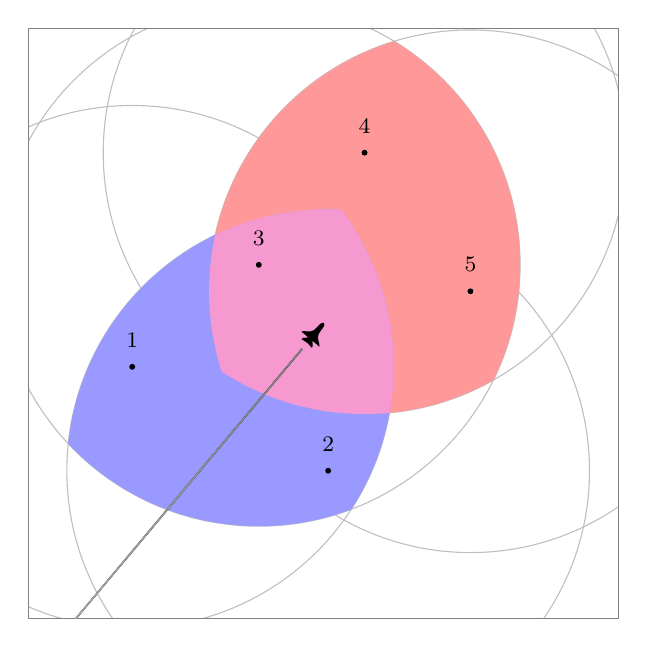
\begin{tikzpicture}[font=\footnotesize,scale=0.9375]
    % Sizes
    \tikzmath{\srange = 3.54; \sradius = 0.04;}
    % Sensor locations (sensor 3 is shared)
    \coordinate (s1) at (1.4086,-4.5869);
    \coordinate (s2) at (4.0633,-5.9948);
    \coordinate (s3) at (3.1235,-3.2054);
    \coordinate (s4) at (4.5563,-1.6861);
    \coordinate (s5) at (5.9909,-3.5635);
    % Navigator location
    \coordinate (nav_loc) at (4,-4);
    % Bounding rectangle
    \coordinate (brect_start) at (0,0);
    \coordinate (brect_end) at (8.0, -8.0);
    
    % Gray range circles
    \begin{scope}
        \clip (brect_start) rectangle (brect_end);
        \draw[gray!50] (s1) circle (\srange);
        \draw[gray!50] (s2) circle (\srange);
        \draw[gray!50] (s3) circle (\srange);
        \draw[gray!50] (s4) circle (\srange);
        \draw[gray!50] (s5) circle (\srange);
    \end{scope}
    % Red subgroup overlap
    \begin{scope}
        \clip (brect_start) rectangle (brect_end);
        \clip (s3) circle (\srange);
        \clip (s4) circle (\srange);
        \clip (s5) circle (\srange);
        \fill[red!40] (brect_start) rectangle (brect_end);
    \end{scope}
    % Blue subgroup overlap
    \begin{scope}
        \clip (brect_start) rectangle (brect_end);
        \clip (s1) circle (\srange);
        \clip (s2) circle (\srange);
        \clip (s3) circle (\srange);
        \fill[blue!40] (brect_start) rectangle (brect_end);
    \end{scope}
    % Magenta double overlap
    \begin{scope}
        \clip (brect_start) rectangle (brect_end);
        \clip (s1) circle (\srange);
        \clip (s2) circle (\srange);
        \clip (s3) circle (\srange);
        \clip (s4) circle (\srange);
        \clip (s5) circle (\srange);
        \fill[magenta!40] (brect_start) rectangle (brect_end);
    \end{scope}
    % Sensors
    \fill[black] (s1) circle (\sradius);
    \fill[black] (s2) circle (\sradius);
    \fill[black] (s3) circle (\sradius);
    \fill[black] (s4) circle (\sradius);
    \fill[black] (s5) circle (\sradius);
    % Bounding box
    \draw[gray] (brect_start) rectangle (brect_end);
    % Navigator
    \clip (brect_start) rectangle (brect_end);
    \begin{scope}[shift={(nav_loc)},rotate=-40,xscale=0.22,yscale=0.3]
        % Plane
        \draw[fill]  plot[smooth, tension=.6] coordinates {
        (-0.65,-0.9) 
        (-0.6,-0.85) 
        (-0.4,-0.75) 
        (-0.25,-0.65) 
        (-0.15,-0.5) 
        (-0.12,-0.3) 
        (-0.10,-0.1) 
        (0.0,0.0) 
        (0.10,-0.1) 
        (0.12,-0.3) 
        (0.15,-0.5) 
        (0.25,-0.65) 
        (0.4,-0.75) 
        (0.6,-0.85) 
        (0.65,-0.9)
        } -- plot[smooth, tension=.6] coordinates {
        (0.65,-0.9) 
        (0.15,-0.91)
        (0.35,-1.1) 
        (0.37,-1.15)
        } -- plot[smooth, tension=.6] coordinates {
        (0.37,-1.15)
        (0.0,-1.12) 
        (-0.37,-1.15) 
        } -- plot[smooth, tension=.6] coordinates {
        (-0.37,-1.15)
        (-0.35,-1.1) 
        (-0.15,-0.91) 
        (-0.65,-0.9) 
        } -- cycle;
        % Trail
        \fill[bottom color=white, top color=gray] (-0.05, -1.5) rectangle (0.05, -50);
    \end{scope}
    % Sensor labels
    \node[label=1] at (s1) {};
    \node[label=2] at (s2) {};
    \node[label=3] at (s3) {};
    \node[label=4] at (s4) {};
    \node[label=5] at (s5) {};
\end{tikzpicture}
\caption{An example of sensor subsets; $\{1,2,3\}$ and $\{3,4,5\}$, and the areas where the navigator is in range of all sensors within a subset.}
\label{fig:sensor_subsets}
\end{figure}

% 
% ##       ########    ###    ##    ##    ###     ######   ######## 
% ##       ##         ## ##   ##   ##    ## ##   ##    ##  ##       
% ##       ##        ##   ##  ##  ##    ##   ##  ##        ##       
% ##       ######   ##     ## #####    ##     ## ##   #### ######   
% ##       ##       ######### ##  ##   ######### ##    ##  ##       
% ##       ##       ##     ## ##   ##  ##     ## ##    ##  ##       
% ######## ######## ##     ## ##    ## ##     ##  ######   ######## 
% 

\subsection{Inherent Leakage}
Leakage of information will be discussed in more detail in Section \ref{subsec:leakage}, however, we stress that in any estimation problem where process and measurement models are known, knowledge of sequential state estimates naturally leads to the leakage of some measurement information. For this reason, we accept that average information about sensors may be leaked at each time step and instead show that individual sensor information remains private.

% 
%  .d8888b.                            888                 8888888b.                  888 d8b               
% d88P  Y88b                           888                 888   Y88b                 888 Y8P               
% 888    888                           888                 888    888                 888                   
% 888        888d888 888  888 88888b.  888888 .d88b.       888   d88P 888d888 .d88b.  888 888 88888b.d88b.  
% 888        888P"   888  888 888 "88b 888   d88""88b      8888888P"  888P"  d8P  Y8b 888 888 888 "888 "88b 
% 888    888 888     888  888 888  888 888   888  888      888        888    88888888 888 888 888  888  888 
% Y88b  d88P 888     Y88b 888 888 d88P Y88b. Y88..88P      888        888    Y8b.     888 888 888  888  888 
%  "Y8888P"  888      "Y88888 88888P"   "Y888 "Y88P"       888        888     "Y8888  888 888 888  888  888 
%                         888 888                                                                           
%                    Y8b d88P 888                                                                           
%                     "Y88P"  888                                                                           
% 

\section{Cryptography Preliminaries} \label{sec:crypto_prelim}
When defining our system security requirements and encryption scheme, we will reference some existing cryptographic security notions, the additively homomorphic Paillier encryption scheme, and the Joye-Libert private aggregation scheme.

% 
%  ######  ########  ######  ##     ## ########  #### ######## ##    ## 
% ##    ## ##       ##    ## ##     ## ##     ##  ##     ##     ##  ##  
% ##       ##       ##       ##     ## ##     ##  ##     ##      ####   
%  ######  ######   ##       ##     ## ########   ##     ##       ##    
%       ## ##       ##       ##     ## ##   ##    ##     ##       ##    
% ##    ## ##       ##    ## ##     ## ##    ##   ##     ##       ##    
%  ######  ########  ######   #######  ##     ## ####    ##       ##    
% 

\subsection{Security Notions}
The security of a cryptographic scheme is typically defined by a security \textit{game}, which captures both the desired privacy guarantees, as well as the capabilities of attackers \cite{katzIntroductionModernCryptography2008}. The typical security notion for a homomorphic encryption scheme is Indistinguishability under Chosen Plaintext Attack (IND-CPA) \cite{chaseSecurityHomomorphicEncryption2017}. 
\begin{defn}
An encryption scheme meets IND-CPA security if an attacker who can choose plaintext messages to be encrypted at will, gains no additional information about an unknown plaintext message when they learn only its encryption. 

The formal security game for IND-CPA has been given in Appendix \ref{app:ind_cpa}.
\end{defn}
Private aggregation schemes aim for the security notion of Aggregator Obliviousness (AO) \cite{shiPrivacyPreservingAggregationTimeSeries2011}. 
\begin{defn}
An encryption scheme meets AO security if no colluding subset of participants \textit{excluding} the aggregator gains additional information about the remaining aggregation values given only their encryptions, while any colluding subset \textit{including} the aggregator learns only their sum. 

The formal security game for AO has been given in Appendix \ref{app:ao}.
\end{defn}

% 
% ########     ###    #### ##       ##       #### ######## ########  
% ##     ##   ## ##    ##  ##       ##        ##  ##       ##     ## 
% ##     ##  ##   ##   ##  ##       ##        ##  ##       ##     ## 
% ########  ##     ##  ##  ##       ##        ##  ######   ########  
% ##        #########  ##  ##       ##        ##  ##       ##   ##   
% ##        ##     ##  ##  ##       ##        ##  ##       ##    ##  
% ##        ##     ## #### ######## ######## #### ######## ##     ## 
% 

\subsection{Paillier Encryption Scheme} \label{subsec:paillier_scheme}
The Paillier encryption scheme \cite{paillierPublicKeyCryptosystemsBased1999} is an additively homomorphic encryption scheme which bases its security on the decisional composite residuosity assumption (DCRA) and meets the security notion of IND-CPA. Key generation of the Paillier scheme is performed by choosing two sufficiently large primes $p$ and $q$, and computing $N=pq$. A generator $g$ is also required for encryption, which is often set to $g=N+1$ when $p$ and $q$ are of equal bit length \cite{katzIntroductionModernCryptography2008}. The public key is defined by $(N, g)$ and secret key by $(p, q)$.

Encryption of a plaintext message $m \in \mathbb{Z}_N$, producing ciphertext $c \in \mathbb{Z}^{*}_{N^2}$, is computed by
\begin{equation}
    c = g^m r^N \pmod{N^2}
\end{equation}
for a randomly chosen $r \in \mathbb{Z}_{N}$. $r^N$ can be considered the noise term which hides the value $g^m \pmod{N^2}$, which due to the scheme construction, is an easily computable discrete logarithm. The decryption of a ciphertext is computed by
\begin{equation}
    m = \frac{L(c^\lambda\pmod{N^2})}{L(g^\lambda\pmod{N^2})} \pmod{N}
\end{equation}
where $\lambda = \mathsf{lcm}(p-1, q-1)$ and $L(u) = \frac{u-1}{N}$.

In addition to encryption and decryption, the following homomorphic functions are provided by the Paillier scheme. $\forall m_1,m_2 \in \mathbb{Z}_N$,
\begin{align}
    \mathcal{D}(\mathcal{E}(m_1)\mathcal{E}(m_2) \hspace{-7pt} \pmod{N^2}) &= m_1+m_2 \hspace{-7pt} \pmod{N} \\
    \mathcal{D}(\mathcal{E}(m_1)g^{m_2} \hspace{-7pt} \pmod{N^2}) &= m_1+m_2\hspace{-7pt}\pmod{N} \\
    \mathcal{D}(\mathcal{E}(m_1)^{m_2} \hspace{-7pt} \pmod{N^2}) &= m_1m_2 \hspace{-7pt} \pmod{N}\,. \label{eqn:paillier_hom_mult}
\end{align}

% 
%       ##         ##    ## 
%       ##          ##  ##  
%       ##           ####   
%       ## #######    ##    
% ##    ##            ##    
% ##    ##            ##    
%  ######             ##    
% 

\subsection{Joye-Libert Private Aggregation Scheme} \label{subsec:joye_libert_scheme}
The Joye-Libert private aggregation scheme \cite{joyeScalableSchemePrivacyPreserving2013} is a scheme defined on time-series data and meets the security notion of AO. Similarly to the Paillier scheme, it bases its security on the DCRA. A notable difference to a public-key encryption scheme is the need for a trusted party to perform an initial key generation and distribution step.

Key generation is computed by choosing two equal length and sufficiently large primes $p$ and $q$, and computing $N=pq$. Additionally, hash function $H:\mathbb{Z} \rightarrow \mathbb{Z}_{N^2}^*$ is defined, and the public key is set to $(N, H)$. $n$ private keys are generated by choosing $sk_i,\,1\leq i\leq n$ uniformly from $\mathbb{Z}_{N^2}$ and distributing them to all users, while the last key is set as
\begin{equation*}
    sk_0 = -\sum^{n}_{i=1}sk_i \pmod{N^2}\,,
\end{equation*}
and sent to the aggregator.

Encryption of plaintext $m^{(t)}_{i} \in \mathbb{Z}_N$ to ciphertext $c^{(t)}_{i} \in \mathbb{Z}_{N^2}$ at time $t$ is computed by user $i$ as
\begin{equation}
    c^{(t)}_{i} = (N+1)^{m^{(t)}_{i}} H(t)^{sk_i} \pmod{N^2}\,,
\end{equation}
where the $H(t)^{sk_i}$ can be considered the noise term which hides the again easily computable discrete logarithm $g^{m^{(t)}_{i}} \pmod{N^2}$, where $g=N+1$.

When all encryptions $c^{(t)}_{i},\,1\leq i \leq n$ are sent to the aggregator, private summation and decryption are computed by the functions
\begin{equation}
    c^{(t)} = H(t)^{sk_0}\prod^{n}_{i=1}c^{(t)}_{i} \pmod{N^2}
\end{equation}
and
\begin{equation}
    \sum^{n}_{i=1}m^{(t)}_{i} = \frac{c^{(t)}-1}{N}\,. \label{eqn:agg_decryption}
\end{equation}
Correctness follows from $\sum^{n}_{i=0}sk_i = 0$, and thus
\begin{equation*}
    \begin{split}
        &H(t)^{sk_0}\prod^{n}_{i=1}c_{i,t} \pmod{N^2} \\
        \equiv &H(t)^{sk_0}\prod^{n}_{i=1}(N+1)^{m_{i,t}} H(t)^{sk_i} \pmod{N^2} \\
        \equiv &H(t)^{\sum^n_{j=0}sk_j} \prod^{n}_{i=1}g^{m_{i,t}} \pmod{N^2} \\
        \equiv &(N+1)^{\sum^n_{i=1}m_{i,t}} \pmod{N^2}
    \end{split}
\end{equation*}
removing all noise terms.

% 
%  .d8888b.                            888                 8888888b.                  888      
% d88P  Y88b                           888                 888   Y88b                 888      
% 888    888                           888                 888    888                 888      
% 888        888d888 888  888 88888b.  888888 .d88b.       888   d88P 888d888 .d88b.  88888b.  
% 888        888P"   888  888 888 "88b 888   d88""88b      8888888P"  888P"  d88""88b 888 "88b 
% 888    888 888     888  888 888  888 888   888  888      888        888    888  888 888  888 
% Y88b  d88P 888     Y88b 888 888 d88P Y88b. Y88..88P      888        888    Y88..88P 888 d88P 
%  "Y8888P"  888      "Y88888 88888P"   "Y888 "Y88P"       888        888     "Y88P"  88888P"  
%                         888 888                                                              
%                    Y8b d88P 888                                                              
%                     "Y88P"  888                                                              
% 

\section{Private Linear-Combination Aggregation} \label{sec:lcao_definition}
For achieving the goal of private localisation defined in Section \ref{sec:problem_statement} we will require a multi-party protocol for computing linear combinations of weights, and their subsequent aggregation. In the context of navigation, $m$ weights $\omega_j^{(t)}, 1 \leq j \leq m$ are first broadcast by the navigator, linear combinations $y^{(t)}_i=\sum^m_{j=1}x_{j,i}^{(t)}\omega_i^{(t)}$ are computed by each sensor $1\leq i\leq n$, and aggregation is computed back at the navigator, at every time step $t$. This has been summarized in Figure \ref{fig:agg_steps}. In Section \ref{sec:private_localisation} we will show how this protocol can be sufficient to compute measurement covariances and measurement vectors, and update the Extended Information Filter.

\begin{figure}[htbp]
\centering
\vspace{\baselineskip}
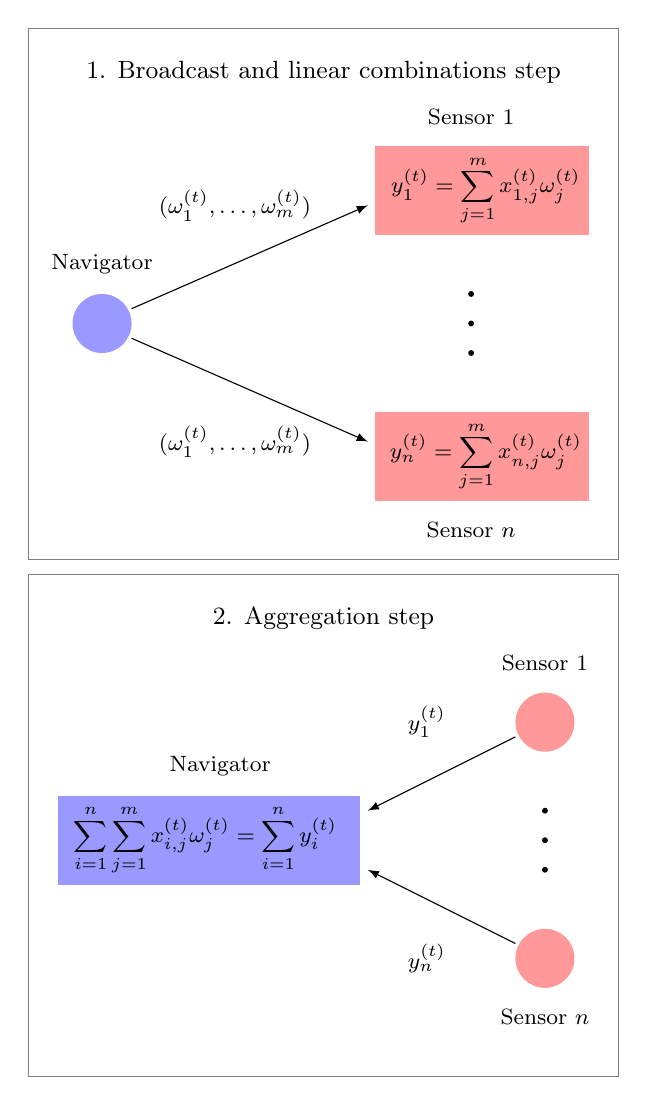
\begin{tikzpicture}[font=\footnotesize,scale=0.75]
    % Step 1
    \node at (5,22.5) {\small 1. Broadcast and linear combinations step};
    % Navigator
    \node at (1.25,19.25) {Navigator};
    \fill (1.25,18.25) [blue!40] ellipse (0.5 and 0.5);
    % Sensors
    \node at (7.5,21.75) {Sensor $1$};
    \fill [red!40] (5.875,19.75) rectangle (9.5,21.25);
    \node at (7.75,20.5) {$\displaystyle y_1^{(t)} = \sum^m_{j=1}x_{1,j}^{(t)}\omega_j^{(t)}$};
    \node at (7.5,14.75) {Sensor $n$};
    \fill [red!40] (5.875,15.25) rectangle (9.5,16.75);
    \node at (7.75,16) {$\displaystyle y_n^{(t)} = \sum^m_{j=1}x_{n,j}^{(t)}\omega_j^{(t)}$};
    \fill [black] (7.5,18.75) circle (0.05);
    \fill [black] (7.5,17.75) circle (0.05);
    \fill [black] (7.5,18.25) circle (0.05);
    % Lines
    \draw [-latex] plot[smooth, tension=.7] coordinates {(1.75,18.5) (5.75,20.25)};
    \draw [-latex] plot[smooth, tension=.7] coordinates {(1.75,18) (5.75,16.25)};
    \node at (3.5,20.25) {$(\omega_1^{(t)},\dots ,\omega_m^{(t)})$};
    \node at (3.5,16.25) {$(\omega_1^{(t)},\dots ,\omega_m^{(t)})$};
    
    % Step 2
    \node at (5,13.25) {\small 2. Aggregation step};
    % Navigator
    \node at (3.25,10.75) {Navigator};
    \fill [blue!40] (0.5,8.75) rectangle (5.625,10.25);
    \node at (3,9.5) {$\displaystyle \sum^{n}_{i=1}\sum^{m}_{j=1} x_{i,j}^{(t)}\omega_j^{(t)} = \sum^n_{i=1}y^{(t)}_{i}$};
    % Sensors
    \node at (8.75,12.5) {Sensor $1$};
    \fill  (8.75,7.5) [red!40] ellipse (0.5 and 0.5);
    \node at (8.75,6.5) {Sensor $n$};
    \fill  (8.75,11.5) [red!40] ellipse (0.5 and 0.5);
    \fill [black] (8.75,10) circle (0.05);
    \fill [black] (8.75,9) circle (0.05);
    \fill [black] (8.75,9.5) circle (0.05);
    % Lines
    \draw [-latex] plot[smooth, tension=.7] coordinates {(8.25,11.25) (5.75,10)};
    \draw [-latex] plot[smooth, tension=.7] coordinates {(8.25,7.75) (5.75,9)};
    \node at (6.75,11.5) {$y_1^{(t)}$};
    \node at (6.75,7.5) {$y_n^{(t)}$};
    
    % Bounding rectangles
    \draw [gray] (0,23.25) rectangle (10,14.25);
    \draw [gray] (0,14) rectangle (10,5.5);
\end{tikzpicture}
\vspace{\baselineskip}
\caption{Required linear-combination aggregation steps at time $t$}
\label{fig:agg_steps}
\end{figure}

To perform the protocol from Figure \ref{fig:agg_steps} in a secure manner, we must first describe the security properties we aim to achieve. Broadly speaking, we want a cryptographic scheme which allows a time-series of homomorphically computed linear combinations of encrypted weights, to be summed by a private aggregation scheme. That is, we do not want sensors to learn the navigator weights, while we do not want the navigator to learn individual weighted linear combinations. This can be summarised by the two informal security notions:
\begin{description}
    \item[Indistinguishable Weights] No colluding subset of sensors gains any additional knowledge about the navigator weights $\omega_j,\,1\leq j \leq m$ from receiving only their encryptions from the current and previous timesteps, and the ability to encrypt plaintexts of their choice.
    \item[Private Linear Combination Aggregation] No colluding subset \textit{excluding} the aggregator gains additional information about the remaining sensor values to be weighted $x^{(t)}_{i,j},\,0\leq j\leq m$, where sensor $i$ is not colluding, given only encryptions of their linear combinations $y_i$ from the current and previous timesteps. Any colluding subset \textit{including} the aggregator learns only the sum of all linear combinations weighted by weights of their choice, $\sum^n_{i=n}\sum^m_{j=1}x^{(t)}_{i,j}\omega^{(t)}_j$.
\end{description}

\begin{rem}
    The notion of a leakage function including parameters from the aggregator requires extra care to be taken when giving its definition. Since an attacker may compromise the aggregator, they have control over the choice of these parameters, and therefore over the leakage function. We note that in the leakage function above, $\sum^n_{i=n}\sum^m_{j=1}x^{(t)}_{i,j}\omega^{(t)}_j$, an individual sum weighted by the same weight may be learned by the colluding subset, \textit{e.g.} $\sum^m_{j=1}x^{(t)}_{1,j}$ given weights $(1,0,\dots,0)$, but that individual sensor values $x^{(t)}_{i,j}$ remain private due to the requirement that all sensors receive the same weights.
\end{rem}

From the informal definitions above, it is clear that weights encrypted by an IND-CPA secure encryption scheme are sufficient for the first requirement, while a scheme satisfying AO is not sufficient for the second. To formalise the second requirement, we define a novel encryption type ``Linear-Combination Aggregator Oblivious Encryption'' and an accompanying security game, which capture the additional weights and modified leakage of AO.

% 
% ##        ######     ###     #######  
% ##       ##    ##   ## ##   ##     ## 
% ##       ##        ##   ##  ##     ## 
% ##       ##       ##     ## ##     ## 
% ##       ##       ######### ##     ## 
% ##       ##    ## ##     ## ##     ## 
% ########  ######  ##     ##  #######  
% 

\subsection{Linear-Combination Aggregator Oblivious Encryption} \label{subsec:lcao}
We let a linear-combination aggregator oblivious encryption scheme be defined as a tuple of the four algorithms $(\mathsf{Setup}, \mathsf{Enc}, \mathsf{CombEnc}, \mathsf{AggDec})$, defined as

\begin{description}
    \item[$\mathsf{Setup}(\kappa)$] On input of security paramater $\kappa$, generate public parameters $\mathsf{pub}$, number of weights $m$, the aggregator's public and private keys $pk_0$ and $sk_0$, and the remaining user private keys $sk_i,\,1\leq i \leq n$.
    \item[$\mathsf{Enc}(pk_0, \omega)$] The aggregator and users can encrypt a weight $\omega$ with the aggregator public key $pk_0$, and obtain the encryption $\mathcal{E}_{pk_0}(\omega)$.
    \item[$\mathsf{CombEnc}(t, pk_0, sk_i, \mathcal{E}_{pk_0}(\omega_1^{(t)}),\dots,\mathcal{E}_{pk_0}(\omega_m^{(t)}), x^{(t)}_{i,1},\dots,x^{(t)}_{i,m})$] At time $t$, user $i$ computes and obtains the encrypted linear combination $y^{(t)}_i = \mathcal{E}_{pk_0,sk_i}(\sum^m_{j=1}x^{(t)}_{i,j}\omega^{(t)}_j)$ using its secret key $sk_i$.
    \item[$\mathsf{AggDec}(t, pk_0, sk_0, y^{(t)}_1,\dots,y^{(t)}_n)$] At time $t$, the aggregator computes the aggregation of linear combinations $\sum^{n}_{i=1}\sum^{m}_{j=1} x^{(t)}_{i,j}\omega^{(t)}_j$ using its public and private keys $pk_0$, $sk_0$.
\end{description}

Next, we formalise the security notion of Linear-Combination Aggregator Obliviousness (LCAO) as the following game between attacker and challenger:

\begin{description}
    \item[Setup] The challenger runs the $\mathsf{Setup}$ algorithm and gives $\mathsf{pub}$, $m$ and $pk_0$ to the attacker
    \item[Queries] The attacker can now perform encryptions or submit queries that are answered by the challenger. The types of actions are:
    \begin{enumerate}
        \item \textit{Encryption:} The attacker chooses a weight $\omega$ and computes an encryption of $\omega$ under the aggregator's public key $pk_0$, obtaining $\mathcal{E}_{pk_0}(\omega)$.
        \item \textit{Weight Queries:} The attacker chooses a time $t$ and receives the weights for that time encrypted with the aggregator's public key, $\mathcal{E}_{pk_0}(\omega^{(t)}_{j}),\,1\leq j\leq m$.
        \item \textit{Combine Queries:} The attacker chooses a tuple $(i,t,x^{(t)}_{i,1},\dots,x^{(t)}_{i,m})$ such that for any two chosen combine query tuples $(i,t,x^{(t)}_{i,1},\dots,x^{(t)}_{i,m})$ and $(i',t',x^{\prime(t')}_{i',1},\dots,x^{\prime(t')}_{i',m})$, the following condition holds:
        \begin{equation*}
            i = i' \wedge t = t' \implies x^{(t)}_{i,m} = x^{\prime(t')}_{i',m},\,1\leq j\leq m\,.
        \end{equation*}
        They are given back the encryption of the linear combination $\mathcal{E}_{pk_0,sk_i}(\sum^m_{j=1}x^{(t)}_{i,j}\omega^{(t)}_j)$ encrypted under both the aggregator public key $pk_0$ and the secret key $sk_i$.
        \item \textit{Compromise queries:} The attacker chooses $i$ and receives the secret key $sk_i$. The aggregator's secret key may also be compromised (when choosing $i=0$).
    \end{enumerate} 
    \item[Challenge] Next, the attacker chooses a time $t^*$, and a subset of users $S \subseteq U$ where $U$ is the complete set of users for which no combine queries, for time $t^*$, and no compromise queries, are made for the duration of the game. The attacker then chooses two series of tuples
    \begin{equation*}
        \langle(i,t^*,x^{(t^*)(0)}_{i,1},\dots,x^{(t^*)(0)}_{i,m})\,|\,i \in S\rangle
    \end{equation*}
    and
    \begin{equation*}
        \langle(i,t^*,x^{(t^*)(1)}_{i,1},\dots,x^{(t^*)(1)}_{i,m})\,|\, i \in S\rangle\,,
    \end{equation*}
    and gives them to the challenger. In the case that $0 \in S$ (\textit{i.e.} the aggregator is compromised) and $S = U$, it is additionally required that
    \begin{equation*}
        \sum_{i\in S}\sum^{m}_{j=1} x^{(t^*)(0)}_{i,j}\omega^{(t^*)}_j = \sum_{i \in S}\sum^{m}_{j=1} x^{(t^*)(1)}_{i,j}\omega^{(t^*)}_j\,,
    \end{equation*}
    for weights $\omega^{(t^*)}_j,\,1\leq j \leq m$ returned by a \textit{Weight Query} with chosen time $t^*$. The challenger then chooses a random bit $b \in \{1,0\}$ and returns encryptions 
    \begin{equation*}
        \langle\mathcal{E}_{pk_0,sk_i}(\sum^m_{j=1}x^{(t^*)(b)}_{i,j}\omega^{(t^*)}_j)\,|\,i\in S\rangle\,.
    \end{equation*}
    \item[More Queries] The attacker can now perform more encryptions and submit queries, so long as the queries do not break the requirements in the Challenge stage. That is, $S \subseteq U$.
    \item[Guess] At the end, the attacker outputs a bit $b'$ and wins the game only if $b' = b$. The advantage of an attacker $\mathcal{A}$ is defined as
    \begin{equation*}
        \mathsf{Adv}^{LCAO}(\mathcal{A}) \coloneqq \left\lvert \Pr [b'=b] - \frac{1}{2}\right\rvert\,.
    \end{equation*} 
\end{description}

\begin{defn}
    An encryption scheme meets LCAO security if no adversary, running in probabilistic-time with respect to security parameter, has more than a negligible advantage in winning the above security game. Probabilities are taken over randomness introduced by $\mathcal{A}$, and in $\mathsf{Setup}$, $\mathsf{Enc}$ and $\mathsf{CombEnc}$.
\end{defn}

In the next section, we will give a solution to an encryption scheme meeting LCAO security, with IND-CPA secure weight encryption, and give a cryptographic proof for its security.

% 
%  .d88888b.                         .d8888b.           888                                      
% d88P" "Y88b                       d88P  Y88b          888                                      
% 888     888                       Y88b.               888                                      
% 888     888 888  888 888d888       "Y888b.    .d8888b 88888b.   .d88b.  88888b.d88b.   .d88b.  
% 888     888 888  888 888P"            "Y88b. d88P"    888 "88b d8P  Y8b 888 "888 "88b d8P  Y8b 
% 888     888 888  888 888                "888 888      888  888 88888888 888  888  888 88888888 
% Y88b. .d88P Y88b 888 888          Y88b  d88P Y88b.    888  888 Y8b.     888  888  888 Y8b.     
%  "Y88888P"   "Y88888 888           "Y8888P"   "Y8888P 888  888  "Y8888  888  888  888  "Y8888  
%                                                                                                
%                                                                                                
%                                                                                                
% 

\section{Our Scheme} \label{sec:our_scheme}
Our scheme is based on the Paillier and Joye-Libert schemes introduced in Section \ref{sec:crypto_prelim}, and similarly bases its security on the DCRA. As with Joye-Libert's private aggregation scheme, a trusted party is required for the initial distribution of user secret keys. Below, we give definitions for the four algorithms comprising the linear-combination aggregation encryption scheme.

\begin{description}
    \item[$\mathsf{Setup}(\kappa)$] On input parameter $\kappa$, generate two equal length, sufficiently large, primes $p$ and $q$, and compute $N=pq$. Define a hash function $H:\mathbb{Z} \rightarrow \mathbb{Z}_{N^2}^*$, choose an $m>1$ as the number of weights to combine, and set public parameter $\mathsf{pub}=H$, aggregator public key $pk_0 = N$ and aggregator private key $sk_0=(p,q)$. The remaining user secret keys are generated by choosing $sk_i,\,1\leq i\leq n-1$ uniformly from $\mathbb{Z}_{N^2}$ and setting the last key as $sk_0 = -\sum^{n}_{i=1}sk_i \pmod{N^2}$.
 
    \item[$\mathsf{Enc}(pk_0, \omega)$] Encryption of weights is computed as a Paillier encryption with implicit generator $g=N+1$. This is given by
    \begin{equation}
        \mathcal{E}_{pk_0}(\omega) = (N+1)^{\omega}r^N \pmod{N^2}\,,
    \end{equation}
    for a randomly chosen $r \in \mathbb{Z}_N$.

    \item[$\mathsf{CombEnc}(t, pk_0, sk_i, \mathcal{E}_{pk_0}(\omega_1^{(t)}),\dots,\mathcal{E}_{pk_0}(\omega_m^{(t)}), x^{(t)}_{i,1},\dots,x^{(t)}_{i,m})$] The linear combination encryption step at time $t$ is computed as 
    \begin{equation}
        y^{(t)}_i = H(t)^{sk_i}\prod^{m}_{j=1}\mathcal{E}_{pk_0}(\omega^{(t)}_j)^{x^{(t)}_{i,j}} \pmod{N^2}\,,\label{eqn:our_scheme_lin_comb}
    \end{equation}
    and makes use of the homomorphic property \eqref{eqn:paillier_hom_mult}. Correctness follows from
    \begin{equation*}
        \begin{split}
             y^{(t)}_i &= H(t)^{sk_i}\prod^{m}_{j=1}\mathcal{E}_{pk_0}(\omega^{(t)}_j)^{x^{(t)}_{i,j}} \pmod{N^2} \\
            &= H(t)^{sk_i}\prod^{m}_{j=1}\mathcal{E}_{pk_0}(x^{(t)}_{i,j}\omega^{(t)}_j) \pmod{N^2} \\
            &= H(t)^{sk_i}\prod^{m}_{j=1}(N+1)^{x^{(t)}_{i,j}\omega^{(t)}_j} r^{N}_{j} \pmod{N^2} \\
            &= H(t)^{sk_i}(N+1)^{\sum^{m}_{j=1}x^{(t)}_{i,j}\omega^{(t)}_j} r_{i}^{N} \pmod{N^2}\,,
        \end{split}
    \end{equation*}
    for some values $r_i,r_j \in \mathbb{Z}_N\,,1\leq j \leq m$. Here, $r_i^N$ and $H(t)^{sk_i}$ can be considered the noise terms corresponding to the two levels of encryption from $pk_0$ and $sk_i$, respectively.

    \item[$\mathsf{AggDec}(t, pk_0, sk_0, y^{(t)}_1,\dots,y^{(t)}_n)$] Aggregation is computed as $y^{(t)} = \prod^n_{i=1}y^{(t)}_i \pmod{N^2}$, removing aggregation noise terms, and is followed by Paillier decryption
    \begin{equation}
        \begin{split}
            \sum^{n}_{i=1}\sum^{m}_{j=1}&x^{(t)}_{i,j}\omega^{(t)}_j =\\
            &\frac{L((y^{(t)})^\lambda\pmod{N^2})}{L((N+1)^\lambda\pmod{N^2})} \pmod{N}\,.
        \end{split}
    \end{equation}
    The correctness of aggregation can be seen from
    \begin{align*}
        y^{(t)} &= \prod^n_{i=1}H(t)^{sk_i}(N+1)^{\sum^{m}_{j=1}x_{i,j}\omega_j}r_i^N \pmod{N^2} \\
        \begin{split}
            &= H(t)^{\sum^n_{i=1}sk_i}\cdot \\
            &\qquad\qquad \prod^n_{i=1}(N+1)^{\sum^{m}_{j=1}x^{(t)}_{i,j}\omega^{(t)}_j}r_i^N \pmod{N^2}
        \end{split}\\
        &= (N+1)^{\sum^n_{i=1}\sum^{m}_{j=1}x^{(t)}_{i,j}\omega^{(t)}_j}r'^N \pmod{N^2}\,,
    \end{align*}
    for some values $r_i,r' \in \mathbb{Z}_N,\,1\leq i \leq n$.
\end{description}

Additionally, we note that in the above construction, all weights $\omega^{(t)}_j$ and values $x^{(t)}_{i,j}$ are integers, and that resulting linear combinations and summations are computed $\pmod{N}$.

% 
% ########  ########   #######   #######  ######## 
% ##     ## ##     ## ##     ## ##     ## ##       
% ##     ## ##     ## ##     ## ##     ## ##       
% ########  ########  ##     ## ##     ## ######   
% ##        ##   ##   ##     ## ##     ## ##       
% ##        ##    ##  ##     ## ##     ## ##       
% ##        ##     ##  #######   #######  ##       
% 

\subsection{Security Proof}
To prove the security of our introduced scheme, we recall the desired security properties of an LCAO secure scheme with IND-CPA secure encrypted weights. From the definition above, weights encrypted with public key $pk_0$ are identical to encryptions of the Paillier scheme, and therefore meet security notion IND-CPA. We omit this proof here and refer readers to the security proof of the Paillier encryption scheme \cite{paillierPublicKeyCryptosystemsBased1999} instead.

To show our scheme meets the security notion of LCAO, we prove by contrapositive that for an adversary $\mathcal{A}$ playing against a challenger using \textit{our scheme}, we can create an adversary $\mathcal{A}'$ playing against a challenger using the \textit{Joye-Libert scheme}, such that
\begin{equation*}
    \mathsf{Adv}^{LCAO}(\mathcal{A}) > \eta_1(\kappa) \implies \mathsf{Adv}^{AO}(\mathcal{A}') > \eta_2(\kappa)\,,
\end{equation*}
for some negligible functions $\eta_1$ and $\eta_2$. (\textit{i.e.} if we assume our scheme is not LCAO secure, then the Joye-Libert scheme is not AO secure.) This is a contradiction to the Joye-Libert AO proof in \cite{joyeScalableSchemePrivacyPreserving2013}, and will thus conclude our proof. The function $H$ used by our scheme is treated as a \textit{random oracle} in the Joye-Libert AO proof and will, therefore, prove our scheme secure in the random oracle model as well.
\begin{pf}
    Consider adversary $\mathcal{A}$ playing the LCAO game defined in Section \ref{subsec:lcao}. The following is a construction of an adversary $\mathcal{A}'$ playing the AO game in Appendix \ref{app:ao} against a challenger $\mathcal{C}$ using the Joye-Libert aggregation scheme from Section \ref{subsec:joye_libert_scheme}.
    \begin{description}
        \item[Setup] When receiving $N$ and $H$ as public parameters from $\mathcal{C}$, choose an $m>1$ and give public parameter $H$, number of weights $m$, and $pk_0=N$ to $\mathcal{A}$.
        \item[Queries] Handle queries from $\mathcal{A}$:
        \begin{description}
            \item[\textit{Weight Query}] When $\mathcal{A}$ submits a weight query $t$, choose weights $\omega^{(t)}_j,\,1 \leq j \leq m$ and random values $r_j \in \mathbb{Z}_N,\,1 \leq j \leq m$, and return encryptions 
            \begin{equation*}
                (N+1)^{\omega^{(t)}_{j}}r_j^N\pmod{N^2},\,1\leq j\leq m
            \end{equation*}
            to $\mathcal{A}$.
            \item[\textit{Combine Query}] When $\mathcal{A}$ submits combine query $(i, t, x^{(t)}_{i,1},\dots,x^{(t)}_{i,m})$, choose weights $\omega^{(t)}_j,1 \leq j \leq m$ if not already chosen for time $t$, and make an AO encryption query $(i, t, \sum^m_{j=1}x^{(t)}_{i,j}\omega^{(t)}_j)$ to $\mathcal{C}$. The received response is of the form $(N+1)^{\sum^m_{j=1}x^{(t)}_{i,j}\omega^{(t)}_j}H(t)^{sk_i}$; multiply it by $r^N$ for a random $r \in \mathbb{Z}_N$ and return 
            \begin{equation*}
                (N+1)^{\sum^m_{j=1}x^{(t)}_{i,j}\omega^{(t)}_j}r^N H(t)^{sk_i} \pmod{N^2}
            \end{equation*}
            to $\mathcal{A}$.
            \item[\textit{Compromise Query}] When $\mathcal{A}$ submits compromise query $i$, make the same compromise query $i$ to $\mathcal{C}$, and return the recieved secret key $sk_i$ to $\mathcal{A}$.
        \end{description}
        \item[Challenge] When $\mathcal{A}$ submits challenge series
        \begin{equation*}
            \langle(i,t^*,x^{(t^*)(0)}_{i,1},\dots,x^{(t^*)(0)}_{i,m})\,|\,i \in S\rangle
        \end{equation*}
        and
        \begin{equation*}
            \langle(i,t^*,x^{(t^*)(1)}_{i,1},\dots,x^{(t^*)(1)}_{i,m})\,|\, i \in S\rangle\,,
        \end{equation*}
        choose weights $\omega^{(t^*)}_j,1 \leq j \leq m$ for time $t^*$ and submit AO challenge series
        \begin{equation*}
            \langle(i,t^*,\sum^m_{j=1}x^{(t^*)(0)}_{i,j}\omega^{(t^*)}_j)\,|\,i \in S\rangle
        \end{equation*}
        and
        \begin{equation*}
            \langle(i,t^*,\sum^m_{j=1}x^{(t^*)(1)}_{i,j}\omega^{(t^*)}_j)\,|\,i \in S\rangle\,,
        \end{equation*}
        to $\mathcal{C}$. The received response if of the form 
        \begin{equation*}
            \langle(N+1)^{\sum^m_{j=1}x^{(t^*)(b)}_{i,j}\omega^{(t^*)}_j}H(t^*)^{sk_i}\,|\,i\in U\rangle\,,
        \end{equation*}
        for an unknown $b \in \{0,1\}$. Multiply series elements by $r_i^N,\,1 \leq i \leq n$ for randomly chosen $r_i \in \mathbb{Z}_N$ and return
        \begin{equation*}
            \langle(N+1)^{\sum^m_{j=1}x^{(t^*)(b)}_{i,j}\omega^{(t^*)}_j}r_i^N H(t^*)^{sk_i}\,|\,i\in U\rangle
        \end{equation*}
        to $\mathcal{A}$.
        \item[Guess] When $\mathcal{A}$ makes guess $b'$, make the same guess $b'$ to $\mathcal{C}$.
    \end{description}

    In the above construction, $\mathcal{C}$ follows the Joye-Libert scheme from Section \ref{subsec:joye_libert_scheme} exactly, and to $\mathcal{A}$, $\mathcal{A}'$ behaves identically to our scheme described in Section \ref{sec:our_scheme}. Since $\mathcal{A}'$ runs in polynomial-time to security parameter when $\mathcal{A}$ does, and no non-neglibile advantage adversary to $\mathcal{C}$ exists \cite{joyeScalableSchemePrivacyPreserving2013}, we conclude that no non-negligible advantage adversary $\mathcal{A}$ exists. That is, there exists a negligible function $\eta$, such that
    \begin{equation*}
        \mathsf{Adv}^{LCAO}(\mathcal{A}) \leq \eta(\kappa)
    \end{equation*}
    for security parameter $\kappa$. \qed
\end{pf}

% 
% 888                            8888888b.                  888 d8b               
% 888                            888   Y88b                 888 Y8P               
% 888                            888    888                 888                   
% 888      .d88b.   .d8888b      888   d88P 888d888 .d88b.  888 888 88888b.d88b.  
% 888     d88""88b d88P"         8888888P"  888P"  d8P  Y8b 888 888 888 "888 "88b 
% 888     888  888 888           888        888    88888888 888 888 888  888  888 
% 888     Y88..88P Y88b.         888        888    Y8b.     888 888 888  888  888 
% 88888888 "Y88P"   "Y8888P      888        888     "Y8888  888 888 888  888  888 
%                                                                                 
%                                                                                 
%                                                                                 
% 

\section{Private Localisation Preliminaries} \label{sec:loc_prelim}
The localisation filter we introduce requires real-valued inputs and functions, and relies on a non-linear measurement model. We make use of a real-number encoding scheme which supports the required homomorphic operations and an algebraic reformulation of the Extended Kalman Filter which reduces the filter update step to use only these operations.

% 
% ######## ##    ##  ######   #######  ########  #### ##    ##  ######   
% ##       ###   ## ##    ## ##     ## ##     ##  ##  ###   ## ##    ##  
% ##       ####  ## ##       ##     ## ##     ##  ##  ####  ## ##        
% ######   ## ## ## ##       ##     ## ##     ##  ##  ## ## ## ##   #### 
% ##       ##  #### ##       ##     ## ##     ##  ##  ##  #### ##    ##  
% ##       ##   ### ##    ## ##     ## ##     ##  ##  ##   ### ##    ##  
% ######## ##    ##  ######   #######  ########  #### ##    ##  ######   
% 

\subsection{Integer Encoding for Real Numbers}
In the encryption scheme introduced, weights and values are restricted to integers and all operations are computed $\pmod{N}$, thus bounding meaningful inputs to $\{x : x \in \mathbb{Z}_N\}$. For this reason, a quantisation and integer mapping method for real numbers is required for their encryption and homomorphic processing. We quantise with a generalised Q number format \cite{oberstarFixedPointRepresentationFractional2007} due to implementation simplicity and applicability.

We define a subset of rational numbers in terms of a range $r \in \mathbb{N}$ and fractional precision $f \in \mathbb{N}$. This contrasts with the common definition given in terms of total bits $a$ and fractional bits $b$ \cite{oberstarFixedPointRepresentationFractional2007,schulzedarupEncryptedCooperativeControl2019,farokhiSecurePrivateControl2017}, but allows for a direct mapping to integer ranges which are not powers of two. Rational subset $\mathbb{Q}_{r,f}$ is given by
\begin{equation*}
    \mathbb{Q}_{r,f} = \left\{q : f^{-1} | q \wedge -\left\lfloor\frac{r}{2}\right\rfloor \leq q < \left\lfloor\frac{r}{2}\right\rfloor \right\}\,,
\end{equation*}
and we quantise any real number $x$ by taking the nearest rational $q \in \mathbb{Q}_{r,f}$. That is, $\argmin_{q\in\mathbb{Q}_{r,f}} |x-q|$. In this form, mapping rationals $\mathbb{Q}_{r,f}$ to the encryption scheme range $\mathbb{Z}_N$ is achieved by choosing $r=N$, and handling negatives with modulo arithmetic. In addition, we note that the Q number format requires a precision factor $f$ to be removed after each encoded multiplication, which is not supported by our encryption scheme. This is captured by a third parameter $m$; the number of \textit{additional} multiplication factors to add or remove from encodings.

The combined quantisation and encoding function $\mathsf{E}_{r,f,m}(x)$ of a given a real number $x \in \mathbb{R}$, integer range $\mathbb{Z}_N$, and the desired scaling for $m$ prior encoded multiplications, is given by
\begin{equation}
    \mathsf{E}_{N,f,m}(x) = \left\lfloor f^{m+1} x \right\rceil \pmod{N}\,. \label{eqn:encode}
\end{equation}
Decoding of an integer $e \in \mathbb{Z}_N$, is given by
\begin{equation}
    \mathsf{E}^{-1}_{N,f,m}(e) \!=\! 
    \begin{dcases}
        \frac{e\hspace{-8pt}\pmod{N}}{f^{m+1}}, &e\hspace{-8pt}\pmod{N} \leq \left\lfloor\frac{N}{2}\right\rfloor \\
        -\frac{N - e\hspace{-8pt}\pmod{N}}{f^{m+1}}, &\text{otherwise} \\
    \end{dcases}.
\end{equation}

This encoding scheme provides the following homomorphic operations,
\begin{equation}
    \begin{split}
        \mathsf{E}_{N,f,m}(a_1) + \mathsf{E}_{N,f,m}(a_2)& \pmod{N} =\\
        &\mathsf{E}_{N,f,m}(a_1+a_2)
    \end{split}
\end{equation}
and
\begin{equation}
    \begin{split}
        \mathsf{E}_{N,f,m}(a_1)\mathsf{E}_{N,f,m}(a_2)& \pmod{N} =\\
        &\mathsf{E}_{N,f,m+1}(a_1a_2)\,,
    \end{split}
\end{equation}
noting that the modulus corresponds with the encrypted homomorphic operations in \eqref{eqn:our_scheme_lin_comb}.

The choice of a high fractional precision $f$ may reduce quantisation errors introduced in \eqref{eqn:encode}, however, risks an overflow following too many multiplications. Given the largest number of expected multiplications $m_{max}$, and the largest expected decoded value $x$, the parameter should be chosen such that the following condition holds
\begin{equation*}
    \left|f^{m_{max}+1}x\right| < \left\lfloor \frac{N}{2} \right\rfloor\,.
\end{equation*}
In practice, $N$ is typically very large ($N>2^{1024}$) and this condition can be ignored.

% 
% ######## #### ######## 
% ##        ##  ##       
% ##        ##  ##       
% ######    ##  ######   
% ##        ##  ##       
% ##        ##  ##       
% ######## #### ##       
% 

\subsection{Extended Information Filter}
The Extended Information Filter (EIF) \cite{maybeckStochasticModelsEstimation1982} is a reformulation of the Extended Kalman Filter (EKF), such that the update equations are simplified to sums of measurement information from each sensor. This requires the conversion of state estimate $\rvec{x}_k$ and estimate covariance $\mat{P}_k$ to the information vector and matrix
\begin{equation}
    \rvec{y}_k = \mat{P}_k^{-1}\rvec{x}_k \quad\textrm{and}\quad \mat{Y}_k = \mat{P}_k^{-1}\,,
\end{equation}
respectively. In this form, the update equations for $n$ measurements at time $k$, given process and measurement models \eqref{eqn:process_model} and \eqref{eqn:measurement_model}, are given by
\begin{equation}
    \rvec{y}_k = \rvec{y}_{k-1} + \sum^n_{i=1}\mat{H}^\top_{k,i} r^{-1}_i (z_{k,i} - h_i(\mean{x}_k) + \mat{H}_{k,i}\mean{x}_k) \label{eqn:eif_info_vec_update}
\end{equation}
and
\begin{equation}
    \mat{Y}_k = \mat{Y}_{k-1} + \sum^n_{i=1}\mat{H}^\top_{k,i} r^{-1}_i \mat{H}_{k,i}\,, \label{eqn:eif_info_mat_update}
\end{equation}
with Jacobian
\begin{equation}
    \mat{H}_{k,i} = \left.\frac{\partial h_i}{\partial \vec{x}}\right|_{\rvec{x}_k} \label{eqn:measurement_jacobian}
\end{equation}
for sensors $1 \leq i \leq n$. The filter's prediction step can be computed by converting information vector $\rvec{y}_k$ and matrix $\mat{Y}_k$ back to state estimate and covariance 
\begin{equation}
    \rvec{x}_k = \mat{Y}_k^{-1}\rvec{y}_k \quad\textrm{and}\quad \mat{P}_k = \mat{Y}_k^{-1}\,,
\end{equation}
before using the normal EKF prediction equations
\begin{equation}
    \rvec{x}_k = \vec{f}(\rvec{x}_{k-1})
\end{equation}
and
\begin{equation}
    \mat{P}_k = \mat{F}_k\mat{P}_{k-1}\mat{F}_k^\top\,,
\end{equation}
with Jacobian
\begin{equation}
    \mat{F}_{k} = \left.\frac{\partial \vec{f}}{\partial \vec{x}}\right|_{\rvec{x}_{k-1}}\,. \label{eqn:jacobian_f}
\end{equation}

% 
% 8888888b.          d8b               888                       
% 888   Y88b         Y8P               888                       
% 888    888                           888                       
% 888   d88P 888d888 888 888  888      888      .d88b.   .d8888b 
% 8888888P"  888P"   888 888  888      888     d88""88b d88P"    
% 888        888     888 Y88  88P      888     888  888 888      
% 888        888     888  Y8bd8P       888     Y88..88P Y88b.    
% 888        888     888   Y88P        88888888 "Y88P"   "Y8888P 
%                                                                
%                                                                
%                                                                
% 

\section{Private Localisation with Privacy-Preserving Sensors} \label{sec:private_localisation}
Given our definitions for the aggregation scheme in Section \ref{sec:our_scheme} and preliminaries in Section \ref{sec:loc_prelim}, we can now construct a localisation method meeting our problem formulation in Section \ref{sec:problem_statement}. We consider a navigator in the presence of $n$ range sensors, running a local filter with update steps computed by equations \eqref{eqn:eif_info_vec_update} and \eqref{eqn:eif_info_mat_update}. Received information from each sensor $i$ consists of the measurement vector
\begin{equation}
    \rvec{i}_{k,i} = \mat{H}^\top_{k,i} r^{-1}_i (\rv{z}_{k,i} - h_i(\rvec{x}_k) + \mat{H}_{k,i}\rvec{x}_k) \label{eqn:measurement_vec}
\end{equation}
and the measurement matrix
\begin{equation}
    \mat{I}_{k,i} = \mat{H}^\top_{k,i} r^{-1}_i \mat{H}_{k,i}\,, \label{eqn:measurement_mat}
\end{equation}
at each time step $k$. In this form, all sensitive sensor information is exclusively found in $\rvec{i}_{k,i}$ and $\mat{I}_{k,i}$. Namely, their measurements $\rv{z}_{k,i}$, measurement variances $r_i$ and locations $\vec{s}_i$; captured in measurement functions $h_i$ and Jacobians $\mat{H}_{k,i}$. 

Normal privacy-preserving aggregation encryption of $\rvec{i}_{k,i}$ and $\mat{I}_{k,i}$ at the sensors would require the navigator to disclose some location information in $\rvec{x}_k$, for the computing of Jacobians $\mat{H}_{k,i}$. Instead, we want to formulate $\rvec{i}_{k,i}$ and $\mat{I}_{k,i}$ such that the sensors can use an LCAO secure encryption scheme, with location information in $\rvec{x}_k$ as weights from the navigator. As was shown in Section \ref{sec:our_scheme}, this guarantees that sensors cannot learn navigator location information $\rvec{x}_k$, and the navigator cannot learn individual sensor values $\rvec{i}_{k,i}$ and $\mat{I}_{k,i}$. From \eqref{eqn:measurement_vec} and \eqref{eqn:measurement_mat} we see that such a reformulation sets requirements on the possible measurement functions $h_i$. 

% 
% ##     ##   ### ##     ## ###      ########  ########  #######   ######  
% ##     ##  ##    ##   ##    ##     ##     ## ##       ##     ## ##    ## 
% ##     ## ##      ## ##      ##    ##     ## ##       ##     ## ##       
% ######### ##       ###       ##    ########  ######   ##     ##  ######  
% ##     ## ##      ## ##      ##    ##   ##   ##       ##  ## ##       ## 
% ##     ##  ##    ##   ##    ##     ##    ##  ##       ##    ##  ##    ## 
% ##     ##   ### ##     ## ###      ##     ## ########  ##### ##  ######  
% 

\subsection{Requirements for the Measurement Model}
From the definition of matrix multiplication, we know that matrices whose elements are linear combinations of weights can be multiplied to produce elements of new linear combinations, with weights dependant only on those from the original matrices. For example, consider dimension $N\times N$ matrices $\mat{A}$ and $\mat{B}$, where element $(i,j)$ in matrix $\mat{A}$ is of the form $\sum_{l=0}^M w_{l,i,j}a_{l,i,j}$ and similarly for matrix $\mat{B}$, form $\sum_{l=0}^M v_{l,i,j}b_{l,i,j}$. If we consider $w_{l,i,j}$ and $v_{l,i,j}$ as the weight terms, we can write element $(i,j)$ of a product matrix $\mat{A}\mat{B}$, with weights dependant only on these, as
\begin{equation}
    \begin{split}
        \sum_{l=0}^N&\left(\left(\sum_{m=0}^M w_{m,i,j}a_{m,i,l}\right)\left(\sum_{m=0}^Mv_{m,i,j}b_{m,l,j}\right)\right) \\
        &=\sum_{l=0}^N\left(\sum_{m=0}^M\sum_{n=0}^M w_{m,i,l}a_{m,i,l}v_{n,l,j}b_{n,l,j}\right) \\
        &=\sum_{l=0}^N\sum_{m=0}^M\sum_{n=0}^M (w_{m,i,l}v_{n,l,j})a_{m,i,l}b_{n,l,j}\,.
    \end{split} \label{eqn:matrix_mult_weights}
\end{equation}
Similarly, scalar multiplication also holds this property. It is therefore sufficient for $h_i$ and $\mat{H}_{k,i}$ to be linear combinations of information private to the navigator, for $\rvec{i}_{k,i}$ and $\mat{I}_{k,i}$ to be as well. Next, we will show how this can be achieved for the specific case of two-dimensional range-only localisation.

% 
%  #######  ########   ######     ##     ##  #######  ########  ######## ##       
% ##     ## ##     ## ##    ##    ###   ### ##     ## ##     ## ##       ##       
% ##     ## ##     ## ##          #### #### ##     ## ##     ## ##       ##       
% ##     ## ########   ######     ## ### ## ##     ## ##     ## ######   ##       
% ##     ## ##     ##       ##    ##     ## ##     ## ##     ## ##       ##       
% ##     ## ##     ## ##    ##    ##     ## ##     ## ##     ## ##       ##       
%  #######  ########   ######     ##     ##  #######  ########  ######## ######## 
% 

\subsection{Localisation Measurement Model} \label{subsec:observation_model}
Recalling the state definition \eqref{eqn:state_def} and two-dimensional measurement model \eqref{eqn:measurement_model}, we can see that $h_i$ \textit{cannot} be rearranged to a linear combination of elements private to the navigator. In addition, the Jacobian of $h_i$,
\begin{equation}
    \mat{H}_{k,i} = 
    \begin{bmatrix}
        \frac{\rv{x}_k - s_x}{\sqrt{(\rv{x}_k - s_x)^2 + (\rv{y}_k - s_y)^2}} \\
        \frac{\rv{y}_k - s_y}{\sqrt{(\rv{x}_k - s_x)^2 + (\rv{y}_k - s_y)^2}} 
    \end{bmatrix}\,,
\end{equation}
cannot be either. Instead, we consider the modified measurement functions
\begin{equation}
    h'_i(\rvec{x}_k) = h_i(\rvec{x}_k)^2\,. \label{eqn:modified_measurement_func}
\end{equation}
A measurement function in this form allows rearrangement to a linear combination of navigator information, and thus of the corresponding modified measurement vector $\rvec{i}'_{k,i}$ and measurement matrix $\mat{I}'_{k,i}$ as well. The modified measurement functions $h'_i$ can be written as
\begin{equation}
    \begin{split}
        h'_i(\rvec{x}_k) &= \left\lVert
        \begin{bmatrix}
            \rv{x}_k & \rv{y}_k
        \end{bmatrix}^\top - \vec{s}_i\right\rVert^2 \\
        &= (\rv{x}_k - s_x)^2 + (\rv{y}_k - s_y)^2 \\
        &= \rv{x}_k^2 + \rv{y}_k^2 -2s_x\rv{x}_k -2s_y\rv{y}_k +s_x^2 +s_y^2
    \end{split}\,,
\end{equation}
and the corresponding Jacobians $\mat{H}'_{k,i}$ as
\begin{equation}
    \mat{H}'_{k,i} = 
    \begin{bmatrix}
        2\rv{x}_k - 2s_x \\
        2\rv{y}_k - 2s_y
    \end{bmatrix}\,.
\end{equation}
The above have been rearranged as linear combinations of the weights $\rv{x}_k^2$, $\rv{y}_k^2$, $\rv{x}_k$ and $\rv{y}_k$, which capture all the required information that is private to the navigator. 

To show how $\rvec{i}'_{k,i}$ and $\mat{I}'_{k,i}$ can be formulated in a similar manner using \eqref{eqn:matrix_mult_weights}, we require the existance of a modified measurement model of the form
\begin{equation}
    \rv{z}'_{k,i} = h'_i(\rvec{x}_k)+\rv{v}'_{k,i}\,, \label{eqn:modified_measurement_model}
\end{equation}
where $\rv{z}'_{k,i}$ is the modified measurement, and noise $\rv{v}'_{k,i}$ is white and Gaussian. The approximation of $\rv{z}'_{k,i}$ and $\rv{r}_{k,i}$ from original measurements and variances $\rv{z}_{k,i}$ and $r_i$ will be shown in Section \ref{subsec:range_measurement_mod}. 

With the existence of \eqref{eqn:modified_measurement_model}, measurement vector and measurement matrix linear combinations can be given by
\begin{equation}
    \begin{split}
        \rvec{i}'_{k,i} &= \mat{H}_{k,i}^{\prime\top} \rv{r}_{k,i}^{-1}(\rv{z}'_{k,i} - h'_i(\rvec{x}_k) + \mat{H}'_{k,i}\rvec{x}_k) \\
        &= 
        \begin{bmatrix}
            \begin{split}
                &(2\rv{r}_{k,i}^{-1})\rv{x}_k^3 + (2\rv{r}_{k,i}^{-1})\rv{x}_k\rv{y}_k^2 + (-\rv{r}_{k,i}^{-1}s_x)\rv{x}_k^2 \\
                &\quad+ (-2\rv{r}_{k,i}^{-1}s_x)\rv{y}_k^2 + (2\rv{r}_{k,i}^{-1}\rv{z}'_{k,i})\rv{x}_k \\
                &\quad+ (-2\rv{r}_{k,i}^{-1}s_x^2)\rv{x}_k + (-2\rv{r}_{k,i}^{-1}s_y^2)\rv{x}_k \\
                &\quad+ (2\rv{r}_{k,i}^{-1}s_x^3) + (2\rv{r}_{k,i}^{-1}s_xs_y^2) \\
                &\quad+ (-2\rv{r}_{k,i}^{-1}s_x \rv{z}'_{k,i})
            \end{split}
            \vspace{5pt}\\
            \begin{split}
                &(2\rv{r}_{k,i}^{-1})\rv{y}_k^3 + (2\rv{r}_{k,i}^{-1})\rv{x}_k^2\rv{y}_k + (-2\rv{r}_{k,i}^{-1}s_y)\rv{x}_k^2 \\
                &\quad+ (-2\rv{r}_{k,i}^{-1}s_y)\rv{y}_k^2 + (2\rv{r}_{k,i}^{-1}\rv{z}'_{k,i})\rv{y}_k \\
                &\quad+ (-2\rv{r}_{k,i}^{-1}s_x^2)\rv{y}_k + (-2\rv{r}_{k,i}^{-1}s_y^2)\rv{y}_k \\
                &\quad+ (2\rv{r}_{k,i}^{-1}s_ys_x^2) + (2\rv{r}_{k,i}^{-1}s_y^3) \\
                &\quad+ (-2\rv{r}_{k,i}^{-1}s_y\rv{z}'_{k,i})
            \end{split}
        \end{bmatrix}
    \end{split} \label{eqn:hrz_linear_comb}
\end{equation}
and
\begin{equation}
    \begin{split}
        \mat{I}'_{k,i} &= \mat{H}_{k,i}^{\prime\top} \rv{r}_{k,i}^{-1}\mat{H}'_{k,i} \\
        &=
        \begin{bmatrix}
            \alpha_{11} & \alpha_{12} \\
            \alpha_{21} & \alpha_{22}
        \end{bmatrix}\,,
    \end{split} \label{eqn:hrh_linear_comb}
\end{equation}
with
\begin{align*}
    \alpha_{11} &= (4\rv{r}_{k,i}^{-1})\rv{x}_k^2 + (-8\rv{r}_{k,i}^{-1}s_x)\rv{x}_k + (4\rv{r}_{k,i}^{-1}s_x^2) \\
    \begin{split}
        \alpha_{12} &= (4\rv{r}_{k,i}^{-1})\rv{x}_k\rv{y}_k + (-4\rv{r}_{k,i}^{-1}s_y)\rv{x}_k + (-4\rv{r}_{k,i}^{-1}s_x)\rv{y}_k \\
        &\qquad+ (4\rv{r}_{k,i}^{-1}s_xs_y)
    \end{split}\\
    \alpha_{21} &= \alpha_{12} \\
    \alpha_{22} &= (4\rv{r}_{k,i}^{-1})\rv{y}_k^2 + (-8\rv{r}_{k,i}^{-1}s_y)\rv{y}_k + (4\rv{r}_{k,i}^{-1}s_y^2)\,.
\end{align*}
The above rearrangements result in $\rvec{i}'_{k,i}$ and $\mat{I}'_{k,i}$ as linear comabinations of the weights $\rv{x}_k^3$, $\rv{y}_k^3$, $\rv{x}_k^2\rv{y}_k$, $\rv{x}_k\rv{y}_k^2$, $\rv{x}_k^2$, $\rv{y}_k^2$, $\rv{x}_k$ and $\rv{y}_k$, which again capture all the required information private to the navigator.

The final step required for the application of our LCAO-secure encryption scheme to the linear combinations \eqref{eqn:hrz_linear_comb} and \eqref{eqn:hrh_linear_comb} is the handling of the scheme's instance-stamp variable $t$, in \eqref{eqn:our_scheme_lin_comb}. As six linear-combination aggregations occur at each time step $k$ (four element in $\mat{I}'_{k,i}$ and two in $\rvec{i}'_{k,i}$), it is required for the security of the scheme that $t$ be unique for each aggregation at each time. This is handled by setting $t$ to the concatenation 
\begin{equation}
    t=k\mathbin\|i\mathbin\|j\mathbin\|b
\end{equation}
for aggregation in row $i$ and column $j$, with $b=0$ for aggregations in $\rvec{i}'_{k,i}$ and $b=1$ otherwise.
\begin{rem}
    The solutions \eqref{eqn:hrz_linear_comb} and \eqref{eqn:hrh_linear_comb} have been derived for two-dimensional localisation, but can be similarly extended to the three-dimensional case. We note however, the additional cost with increasing dimension. The number of weights is increased in the rearranged functions $h'_i$, and therefore combinatorially increased in $\rvec{i}'_{k,i}$ and $\mat{I}'_{k,i}$ by \eqref{eqn:matrix_mult_weights}. This results in a combinatorial increase in weights, and therefore communication, with respect to the number of state parameters required for computing functions $h_i$.
\end{rem}

% 
%  ######   #######  ##     ##    ###    ########  ######## ########     ######## 
% ##    ## ##     ## ##     ##   ## ##   ##     ## ##       ##     ##         ##  
% ##       ##     ## ##     ##  ##   ##  ##     ## ##       ##     ##        ##   
%  ######  ##     ## ##     ## ##     ## ########  ######   ##     ##       ##    
%       ## ##  ## ## ##     ## ######### ##   ##   ##       ##     ##      ##     
% ##    ## ##    ##  ##     ## ##     ## ##    ##  ##       ##     ##     ##      
%  ######   ##### ##  #######  ##     ## ##     ## ######## ########     ######## 
% 

\subsection{Range Measurement Modification} \label{subsec:range_measurement_mod}
In Section \ref{subsec:observation_model}, we assumed the existance of modified sensor measurements $\rv{z}'_{k,i}$ with Gaussian noise and variances $\rv{r}_{k,i}$ in the modified measurement model \eqref{eqn:modified_measurement_model}. In practice, conversion of range measurements $\rv{z}_{k,i}$ to $\rv{z}'_{k,i}$ is complicated by the noise term $\rv{v}_{k,i} \sim \mathcal{N}(0, r_i)$ in \eqref{eqn:measurement_model}. Squaring the range measurement produces
\begin{equation}
    \begin{split}
        \rv{z}_{k,i}^2 &= (h_i(\rvec{x}_k) + \rv{v}_{k,i})^2 \\
        &= h_i(\rvec{x}_k)^2 + 2h_i(\rvec{x}_k)\rv{v}_{k,i} + \rv{v}_{k,i}^2 \\
        &= h'_i(\rvec{x}_k) + 2h_i(\rvec{x}_k)\rv{v}_{k,i} + \rv{v}_{k,i}^2\,,
    \end{split}
\end{equation}
with new noise term, $2h_i(\rvec{x}_k)\rv{v}_{k,i} + \rv{v}_{k,i}^2$, now dependant on the measurement function $h_i$ and no longer white or Gaussian. We can compute the mean of the new noise term (a function of white Gaussian term $\rv{v}_{k,i}$) as
\begin{equation}
    \E{2h_i(\rvec{x}_k)\rv{v}_{k,i} + \rv{v}_{k,i}^2} = r_i\, \label{eqn:modified_noise_mean}
\end{equation}
and define modified measurements as
\begin{equation} \label{eqn:modified_measurement}
    \begin{split}
        \rv{z}'_{k,i} &= \rv{z}_{k,i}^2 - r_i \\
        &= h_i(\rvec{x}_k)^2 + 2h_i(\rvec{x}_k)\rv{v}_{k,i} + \rv{v}_{k,i}^2 - r_i \\
        &= h'_i(\rvec{x}_k) + \rv{v}'_{k,i}\,,
    \end{split}
\end{equation}
with now zero-mean noise $\rv{v}'_{k,i} = 2h_i(\rvec{x}_k)\rv{v}_{k,i} + \rv{v}_{k,i}^2 - r_i$. The noise in this case (again a function of white Gaussian term $\rv{v}_{k,i}$) has variance 
\begin{equation}
    \Var{\rv{v}'_{k,i}} = 4h_i(\rvec{x}_k)^2r_i + 2r_i^2
\end{equation}
and is dependant on $h_i(\rvec{x}_k)$. We also wish to approximate this noise using values available to the sensor, $\rv{z}_{k,i}$ and $r_i$, while providing a conservative estimate of the true variance so as not to affect the convergence of the EIF. While replacing $h_i(\rvec{x}_k)$ with $\rv{z}_{k,i}$ only provides a conservative estimate in the case
\begin{equation}
    \begin{split}
        \rv{z}_{k,i} &> h_i(\rvec{x}_k) \\
        \rv{z}_{k,i} - h_i(\rvec{x}_k) &> 0 \\
        \rv{v}_{k,i} &> 0\,,
    \end{split}
\end{equation}
which cannot be guaranteed, we can instead provide a conservative estimate with $95\%$ confidence, by shifting measurement $\rv{z}_{k,i}$ by two standard deviations $\sqrt{r_i}$. Thus, the modified measurement variance for sensor $i$ at time $k$ is conservatively approximated by
\begin{equation}
    \rv{r}_{k, i} = 4(\rv{z}_{k,i} + 2\sqrt{r_i})^2r_i + 2r_i^2\,. \label{eqn:modified_meaasurement_variance_estimate}
\end{equation}

In addition, we note that the distribution of noise in \eqref{eqn:modified_measurement} approaches a Gaussian when true ranges are sufficiently larger than measurement variances, as shown by
\begin{equation}
    \begin{split}
        &r_i << h_i(\rvec{x}_k) \\
        \implies &2h_i(\rvec{x}_k)\rv{v}_{k,i} + \rv{v}_{k,i}^2 - r_i \approx 2h_i(\rvec{x}_k)\rv{v}_{k,i} \\
        \implies &\rv{v}'_{k,i} \approx 2h_i(\rvec{x}_k)\rv{v}_{k,i}\,,
    \end{split} \label{eqn:modified_noise_approaches_gaussian}
\end{equation}
and conclude with the following assumption.
\begin{assum}
    Given property \eqref{eqn:modified_noise_approaches_gaussian}, and our $95\%$ confindence in the conservativness of variance estimates \eqref{eqn:modified_meaasurement_variance_estimate}, we assume that range measurements $\rv{z}_i$ are in general large enough to produce sufficiently Gaussian modified measurement noise $\rv{v}'_{k,i}$ and its variance estimated sufficiently conservative to be used in the EIF and measurement model \eqref{eqn:modified_measurement_model}.
\end{assum}

% 
%    ###    ##        ######    #######  ########  #### ######## ##     ## ##     ## 
%   ## ##   ##       ##    ##  ##     ## ##     ##  ##     ##    ##     ## ###   ### 
%  ##   ##  ##       ##        ##     ## ##     ##  ##     ##    ##     ## #### #### 
% ##     ## ##       ##   #### ##     ## ########   ##     ##    ######### ## ### ## 
% ######### ##       ##    ##  ##     ## ##   ##    ##     ##    ##     ## ##     ## 
% ##     ## ##       ##    ##  ##     ## ##    ##   ##     ##    ##     ## ##     ## 
% ##     ## ########  ######    #######  ##     ## ####    ##    ##     ## ##     ## 
% 

\subsection{Algorithm}
% Maybe name the scheme? That would be in the heading here
Piece together the whole algorithm here.
Give the algorithm as pseudocode (including encoding and encryption, possible as separate procedures)

% assume f known to all, and public/private keys already distributed
% Note the abbreviation for encoding E (no N and f)
% Note the different m using in Encoding when computing alphas and betas

\begin{algorithm}
    \caption{Navigator Prediction Step}\label{alg:nav_prediction}
    \begin{algorithmic}[1]
        \Procedure{Prediction}{$\rvec{x}_{k-1}$, $\mat{P}_{k-1}$, $\vec{f}$, $\mat{Q}$, $N$}
        \State Compute $\mat{F}_k$ by \eqref{eqn:jacobian_f}
        \State $\rvec{x}_{k} \gets \vec{f}(\rvec{x}_{k-1})$
        \State $\mat{P}_{k} \gets \mat{F}_k\mat{P}_{k-1}\mat{F}_k^\top + \mat{Q}$
        \For{$\rv{\omega}$ in $\langle\rv{x}_k^3,\rv{y}_k^3,\rv{x}_k^2\rv{y}_k,\rv{x}_k\rv{y}_k^2,\rv{x}_k^2,\rv{y}_k^2,\rv{x}_k,\rv{y}_k\rangle$} 
            \State Compute $\mathsf{E}_{0}(\rv{\omega})$ by \eqref{eqn:encode}
            \State $r \gets$ \Call{RandInt}{$1,N$}
            \State $\mathcal{E}_{pk}(\mathsf{E}_{0}(\rv{\omega})) \gets (N+1)^{\mathsf{E}_{0}(\rv{\omega})}r^N \pmod{N^2}$
            \State Broadcast $\mathcal{E}_{pk}(\mathsf{E}_{0}(\rv{\omega}))$ to sensors
        \EndFor
        \State \Return $\rvec{x}_{k}, \mat{P}_{k}$
        \EndProcedure
    \end{algorithmic}
\end{algorithm}

\begin{algorithm}
    \caption{Measurement at Sensor $i$}\label{alg:measurement_info}
    \begin{algorithmic}[1]
        \Procedure{Measurement}{$i$, $s_x$, $s_y$, $r_i$, $N$, $H$}
        \State Measure $\rv{z}_{k,i}$
        \State Compute $\rv{z}_{k,i}'$ by \eqref{eqn:modified_measurement}
        \State Compute $\rv{r}_{k, i}$ by \eqref{eqn:modified_meaasurement_variance_estimate}
        \While{Navigator broadcasting}
        \State Recieve $\mathcal{E}_{pk}(\mathsf{E}_{0}(\rv{x}^3_k))$
        \State Recieve remaining weights in the form above
        \EndWhile
        \State Let $\beta_{ij}$ represent element $(i,j)$ of $\rvec{i}'_{k,i}$ in \eqref{eqn:hrz_linear_comb}
        \State $\beta_{11} \!\gets\! \mathcal{E}_{pk}(\mathsf{E}_{0}(\rv{x}^3_k))^{\mathsf{E}_{0}(2\rv{r}_{k, i}^{-1})}
        \mathcal{E}_{pk}(\mathsf{E}_{0}(\rv{x}_k\rv{y}^2_k))^{\mathsf{E}_{0}(2\rv{r}_{k, i}^{-1})}$\par
        \ $\mathcal{E}_{pk}(\mathsf{E}_{0}(\rv{x}^2_k))^{\mathsf{E}_{0}(-\rv{r}_{k, i}^{-1}s_x)}
        \mathcal{E}_{pk}(\mathsf{E}_{0}(\rv{y}^2_k))^{\mathsf{E}_{0}(-2\rv{r}_{k, i}^{-1}s_x)}$\par
        \ $\mathcal{E}_{pk}(\mathsf{E}_{0}(\rv{x}_k))^{\mathsf{E}_{0}(2\rv{r}_{k, i}^{-1}\rv{z}_{k,i}')}
        \mathcal{E}_{pk}(\mathsf{E}_{0}(\rv{x}_k))^{\mathsf{E}_{0}(-2\rv{r}_{k, i}^{-1}s_x^2)}$\par
        \ $\mathcal{E}_{pk}(\mathsf{E}_{0}(\rv{x}_k))^{\mathsf{E}_{0}(-2\rv{r}_{k, i}^{-1}s_y^2)}
        (N+1)^{\mathsf{E}_{1}(2\rv{r}_{k, i}^{-1}s_x^3)}$\par
        \ $(N+1)^{\mathsf{E}_{1}(2\rv{r}_{k, i}^{-1}s_xs_y^2)}
        (N+1)^{\mathsf{E}_{1}(-2\rv{r}_{k, i}^{-1}s_x\rv{z}_{k,i}')}$\par
        \ $H(k\mathbin\|1\mathbin\|1\mathbin\|0)\pmod{N^2}$
        \State Compute $\beta_{21}$ by \eqref{eqn:hrz_linear_comb} in the form above
        \For{$i \gets 1$ to $2$}
            \State Send $\beta_{i1}$ to the navigator
        \EndFor
        \State Let $\alpha_{ij}$ represent element $(i,j)$ of $\mat{I}'_{k,i}$ in \eqref{eqn:hrh_linear_comb}
        \State $\alpha_{11} \gets \mathcal{E}_{pk}(\mathsf{E}_{0}(\rv{x}^2_k))^{\mathsf{E}_{0}(4\rv{r}_{k, i}^{-1})}$\par
        \ $\mathcal{E}_{pk}(\mathsf{E}_{0}(\rv{x}_k))^{\mathsf{E}_{0}(-8\rv{r}_{k, i}^{-1}s_x)}
        (N+1)^{\mathsf{E}_{1}(4\rv{r}_{k, i}^{-1}s_x^2)}$\par
        \ $H(k\mathbin\|1\mathbin\|1\mathbin\|1)\pmod{N^2}$
        \State Compute remaining $\alpha_{ij}$ by \eqref{eqn:hrh_linear_comb} in the form above
        \For{$i \gets 1$ to $2$}
            \For{$j \gets 1$ to $2$} 
                \State Send $\alpha_{ij}$ to the navigator
            \EndFor
        \EndFor
        \EndProcedure
    \end{algorithmic}
\end{algorithm}

\begin{algorithm}
    \caption{Navigator Update Step}\label{alg:nav_update}
    \begin{algorithmic}[1]
        \Procedure{Update}{$\rvec{x}_{k}$, $\mat{P}_{k}$, $N$, $\lambda$}
        
        \State Compute $\mat{F}_k$ by \eqref{eqn:jacobian_f}
        \State $\rvec{x}_{k} \gets \vec{f}(\rvec{x}_{k-1})$
        \State $\mat{P}_{k} \gets \mat{F}_k\mat{P}_{k-1}\mat{F}_k^\top + \mat{Q}$
        \For{$\rv{\omega}$ in $\langle\rv{x}_k^3,\rv{y}_k^3,\rv{x}_k^2\rv{y}_k,\rv{x}_k\rv{y}_k^2,\rv{x}_k^2,\rv{y}_k^2,\rv{x}_k,\rv{y}_k\rangle$} 
            \State Compute $\mathsf{E}_{0}(\rv{\omega})$ by \eqref{eqn:encode}
            \State $r \gets$ \Call{RandInt}{$1,N$}
            \State $\mathcal{E}_{pk}(\mathsf{E}_{0}(\rv{\omega})) \gets (N+1)^{\mathsf{E}_{0}(\rv{\omega})}r^N \pmod{N^2}$
            \State Broadcast $\mathcal{E}_{pk}(\mathsf{E}_{0}(\rv{\omega}))$ to sensors
        \EndFor
        \State \Return $\rvec{x}_{k}, \mat{P}_{k}$
        \EndProcedure
    \end{algorithmic}
\end{algorithm}


% 
% ##       ########    ###    ##    ##    ###     ######   ######## 
% ##       ##         ## ##   ##   ##    ## ##   ##    ##  ##       
% ##       ##        ##   ##  ##  ##    ##   ##  ##        ##       
% ##       ######   ##     ## #####    ##     ## ##   #### ######   
% ##       ##       ######### ##  ##   ######### ##    ##  ##       
% ##       ##       ##     ## ##   ##  ##     ## ##    ##  ##       
% ######## ######## ##     ## ##    ## ##     ##  ######   ######## 
% 

\subsection{Leakage} \label{subsec:leakage}
We recall the assumptions made in the problem formulation and our encryption scheme, and the allowed leakage of the encryption scheme. Sensors are honest but curious, meaning sensor values cannot be modified from what is measured, and the protocol is followed exactly, and that the navigator sends the same state information to all sensors at each time step. This is justified to an extent with wireless broadcasting being received by all sensors in a typical localisation setting.

From the above restrictions, sensors learn only their measurements $x_i$, and the navigator learns only the sums $\sum^n_{i=1}H^\top R^{-1}_i(z_i - h(x) + Hx)$ and $\sum^n_{i=1}H^\top R_i^{-1}H$.

For malicious subsets not including the navigator, it is clear that they learn nothing more about the navigator location than what they can deduce given only their own measurements.

The navigator, which may maliciously choose weights at every time step, is always restricted to learning at most the sum $\sum^n_{i=1} a_i$ for some values $a_i$ derived from sensor $i$'s location and measurement. It is therefore intuitive to say that at most the navigator can learn the average of values kept private, that is, the navigator can at most learn the average position and location of sensors. The same can be said for any corrupted subset of honest but curious sensors and malicious navigator.


% 
% 8888888b.                            888 888             
% 888   Y88b                           888 888             
% 888    888                           888 888             
% 888   d88P .d88b.  .d8888b  888  888 888 888888 .d8888b  
% 8888888P" d8P  Y8b 88K      888  888 888 888    88K      
% 888 T88b  88888888 "Y8888b. 888  888 888 888    "Y8888b. 
% 888  T88b Y8b.          X88 Y88b 888 888 Y88b.       X88 
% 888   T88b "Y8888   88888P'  "Y88888 888  "Y888  88888P' 
%                                                          
%                                                          
%                                                          
% 

\section{Results} \label{sec:results}
Time results can be captured in one graph. Y-axis is time, X-axis is the number of sensors, each line (different colour) will show how the runtime changes as sensors are increased for different Paillier bit-sizes (at least 3: 512, 1024, 2048). Every data point should be the average over some X number of simulations.

Accuracy plots will describe error due to encoding and the average distance of the sensors to the navigator. All plots will use the same ground truth and initial state and covariance estimates (this way average error at each timestep from multiple runs makes sense):

Plot 1 will plot the RMSE of the average of X runs at each encoding size. A fixed layout of 4 mediumly spaced sensor will be used, and a fixed Paillier bit size.

Plot 2 will plot the RMSE as the average distance of sensors changes. Fixed encoding and Paillier bit size. Vary between 4 layouts where 4 sensors are either very close to the centre (and ground truth, and progressively further out)

Plot 3 will accompany plot 3 and display the 4 layouts (arrow for ground truth and points for the sensors).

Discuss the meaning of the small changes in accuracy, and runtimes when using the same encryption size, that is, point out it is a generally robust method.

% 
%  .d8888b.                             
% d88P  Y88b                            
% 888    888                            
% 888         .d88b.  88888b.   .d8888b 
% 888        d88""88b 888 "88b d88P"    
% 888    888 888  888 888  888 888      
% Y88b  d88P Y88..88P 888  888 Y88b.    
%  "Y8888P"   "Y88P"  888  888  "Y8888P 
%                                       
%                                       
%                                       
% 

\section{Conclusion} \label{sec:conclusion}
Possible future work to consider: Hardware implementations, measurement handling which preservers Gaussian noise, or non-Gaussian noise methods, ways of sending less information form the navigator to the sensors at each time step, active sensor attacker model, different state encryptions received at sensors or a way to confirm they are the same.

%---Rest is template---


% \section{Introduction}
% Video, patres conscripti, in me omnium vestrum ora atque oculos esse 
% conversos, video vos non solunn de vestro ac rei publicae, verum 
% etiam, si id depulsum sit, de meo periculo esse sollicitos. Est mihi 
% iucunda in malis et grata in dolore vestra erga me voluntas, sed eam, 
% per deos inmortales, deponite atque obliti salutis meae de vobis ac 
% de vestris liberis cogitate. Mihi si haec condicio consulatus data 
% est, ut omnis acerbitates, onunis dolores cruciatusque perferrem, 
% feram non solum fortiter, verum etiam lubenter, dum modo meis 
% laboribus vobis populoque Romano dignitas salusque pariatur.

% \begin{figure}
% \begin{center}
% 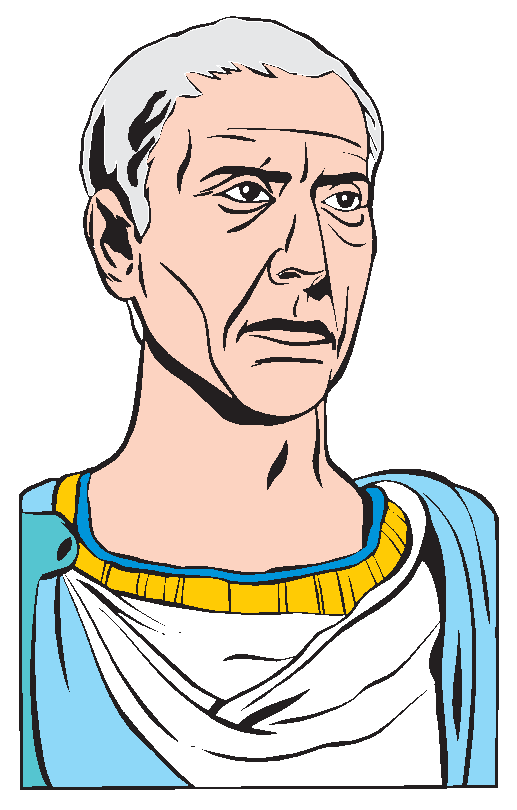
\includegraphics[height=4cm]{jcaesar.eps}    % The printed column  
% \caption{Gaius Julius Caesar, 100--44 B.C.}  % width is 8.4 cm.
% \label{fig1}                                 % Size the figures 
% \end{center}                                 % accordingly.
% \end{figure}

% % OR

% %\begin{figure}
% %\begin{center}
% %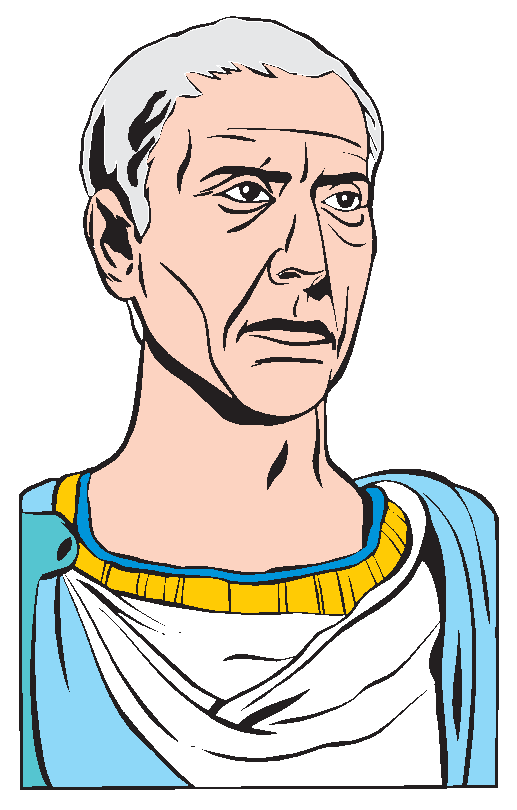
\epsfig{file=jcaesar,width=7cm}
% %\caption{Gaius Julius Caesar, 100--44 B.C.}
% %\label{fig1}
% %\end{center}
% %\end{figure}


% \subsection{A subsection}
% Marcus Tullius Cicero, 106--43 B.C. was a Roman statesman, orator, 
% and philosopher.  A major figure in the last years of the Republic, 
% he is best known for his orations against Catiline\footnote{
% This footnote should be very brief.}
% and for his mastery of Latin prose \cite{Heritage:92}. He was a 
% contemporary of Julius Caesar (Fig.~\ref{fig1}).

% \section{The argument}
% Some words might be appropriate describing equation~(\ref{e1}), if 
% we had but time and space enough.
% \begin{equation} \label{e1}
% {{\partial F}\over {\partial t}} =
% D{{\partial^2 F}\over {\partial x^2}}.
% \end{equation}
% See \cite{Abl:56}, \cite{AbTaRu:54}, \cite{Keo:58} and 
% \cite{Pow:85}.
% This equation goes far beyond the celebrated theorem ascribed to the great
% Pythagoras by his followers.
% \begin{thm}
% The square of the length of the hypotenuse of a right triangle equals the sum of the squares 
% of the lengths of the other two sides.
% \end{thm}
% \section{Epilogue}
% A word or two to conclude, and this even includes some inline 
% maths:  $R(x,t)\sim t^{-\beta}g(x/t^\alpha)\exp(-|x|/t^\alpha)$.

% Place acknowledgements
% here.
\begin{ack}                               
Partially supported by zim
\end{ack}

% Include this if you use bibtex 
% and a bib file to produce the 
% bibliography (preferred). The
% correct style is generated by
% Elsevier at the time of printing.
\bibliographystyle{plain}
\bibliography{BibTeX/PrivateEIFLocalisation}

%\begin{thebibliography}{99}     % Otherwise use the  
                                 % thebibliography environment.
                                 % Insert the full references here.
                                 % See a recent issue of Automatica 
                                 % for the style.
%  \bibitem[Heritage, 1992]{Heritage:92}
%     (1992) {\it The American Heritage. 
%     Dictionary of the American Language.}
%     Houghton Mifflin Company.
%  \bibitem[Able, 1956]{Abl:56}
%     B.~C.~Able (1956). Nucleic acid content of macroscope. 
%     {\it Nature 2}, 7--9. 
%  \bibitem[Able {\em et al.}, 1954]{AbTaRu:54}   
%     B.~C. Able, R.~A. Tagg, and M.~Rush (1954).
%     Enzyme-catalyzed cellular transanimations.
%     In A.~F.~Round, editor, 
%     {\it Advances in Enzymology Vol. 2} (125--247). 
%     New York, Academic Press.
%  \bibitem[R.~Keohane, 1958]{Keo:58}
%     R.~Keohane (1958).
%     {\it Power and Interdependence: 
%     World Politics in Transition.}
%     Boston, Little, Brown \& Co.
%  \bibitem[Powers, 1985]{Pow:85}
%     T.~Powers (1985).
%     Is there a way out?
%     {\it Harpers, June 1985}, 35--47.

%\end{thebibliography}

% Each appendix must have a short title.
% Sections and subsections are supported
% in the appendices.
\appendix
% 
%        d8888                                          888 d8b          
%       d88888                                          888 Y8P          
%      d88P888                                          888              
%     d88P 888 88888b.  88888b.   .d88b.  88888b.   .d88888 888 888  888 
%    d88P  888 888 "88b 888 "88b d8P  Y8b 888 "88b d88" 888 888 `Y8bd8P' 
%   d88P   888 888  888 888  888 88888888 888  888 888  888 888   X88K   
%  d8888888888 888 d88P 888 d88P Y8b.     888  888 Y88b 888 888 .d8""8b. 
% d88P     888 88888P"  88888P"   "Y8888  888  888  "Y88888 888 888  888 
%              888      888                                              
%              888      888                                              
%              888      888                                              
% 

\section{Indistinguishability under Chosen Plaintext Attack (IND-CPA)} \label{app:ind_cpa}
A public-key encryption scheme is defined by the tuple of algorithms $(\mathsf{Setup}, \mathsf{Enc}, \mathsf{Dec})$, defined as
\begin{description}
    \item[$\mathsf{Setup}(\kappa)$] On input of security paramater $\kappa$, generate public key $pk$ and secret key $sk$
    \item[$\mathsf{Enc}(pk, x)$] Encryption of value $x$ is computable using the public key $pk$, obtaining $\mathcal{E}_{pk}(x)$.
    \item[$\mathsf{Dec}(sk, \mathcal{E}_{pk}(x))$] Decryption of value $x$ is computable using the secret key $sk$.
\end{description}

The security game between attacker and challenger for IND-CPA is given by
\begin{description}
    \item[Setup] The challenger runs the $\mathsf{Setup}$ algorithm and gives public key $pk$ to the attacker
    \item[Encryptions] The attacker may compute encryptions using the public key $pk$.
    \item[Challenge] Next, the attacker chooses two values
    \begin{equation*}
        x^{(0)} \text{ and } x^{(1)}
    \end{equation*}
    and gives them to the challenger. The challenger then chooses a random bit $b \in \{1,0\}$ and returns the encryption
    \begin{equation*}
        \mathcal{E}_{pk}(x^{(b)}).
    \end{equation*}
    \item[More Encryptions] The attacker can now compute more encryptions with the public key $pk$.
    \item[Guess] At the end, the attacker outputs a bit $b'$ and wins the game only if $b' = b$. The advantage of an attacker $\mathcal{A}$ is defined as
    \begin{equation*}
        \mathsf{Adv}^{IND-CPA}(\mathcal{A}) \coloneqq \left\lvert \Pr [b'=b] - \frac{1}{2}\right\rvert\,.
    \end{equation*} 
\end{description}

\section{Aggregator Obliviousness (AO)} \label{app:ao}
An aggregator oblivious encryption scheme is defined by the tuple of algorithms $(\mathsf{Setup}, \mathsf{Enc}, \mathsf{AggDec})$, defined as
\begin{description}
    \item[$\mathsf{Setup}(\kappa)$] On input of security paramater $\kappa$, generate public parameters $\mathsf{pub}$, the user private keys $sk_i,\,1\leq i \leq n$, and the aggregator's private key $sk_0=-\sum^n_{i=1}sk_i$.
    \item[$\mathsf{Enc}(t, sk_i, x^{(t)}_i)$] At time $t$, user $i$ computes and obtains the encrypted value $y^{(t)}_i = \mathcal{E}_{sk_i}(x^{(t)}_i)$ using its secret key $sk_i$.
    \item[$\mathsf{AggDec}(t, sk_0, y^{(t)}_1,\dots,y^{(t)}_n)$] At time $t$, the aggregator computes the aggregation of values $\sum^{n}_{i=1} x^{(t)}_i$ using its private key $sk_0$.
\end{description}

The security game between attacker and challenger for AO is given by
\begin{description}
    \item[Setup] The challenger runs the $\mathsf{Setup}$ algorithm and gives public parameters $\mathsf{pub}$ to the attacker
    \item[Queries] The attacker can now submit queries that are answered by the challenger. The types of queries are:
    \begin{enumerate}
        \item \textit{Combine Queries:} The attacker chooses a tuple $(i,t,x^{(t)}_i$ such that for any two chosen combine query tuples $(i,t,x^{(t)}_i)$ and $(i',t',x^{\prime(t')}_{i'}$, the following condition holds:
        \begin{equation*}
            i = i' \wedge t = t' \implies x^{(t)}_{i} = x^{\prime(t')}_{i'}\,.
        \end{equation*}
        They are given back the encryption of the value $\mathcal{E}_{sk_i}(x^{(t)}_i)$ encrypted under the secret key $sk_i$.
        \item \textit{Compromise queries:} The attacker chooses $i$ and receives the secret key $sk_i$. The aggregator's secret key may also be compromised (when choosing $i=0$).
    \end{enumerate} 
    \item[Challenge] Next, the attacker chooses a time $t^*$, and a subset of users $S \subseteq U$ where $U$ is the complete set of users for which no combine queries, for time $t^*$, and no compromise queries, are made for the duration of the game. The attacker then chooses two series of tuples
    \begin{equation*}
        \langle(i,t^*,x^{(t^*)(0)}_i)\,|\,i \in S\rangle
    \end{equation*}
    and
    \begin{equation*}
        \langle(i,t^*,x^{(t^*)(1)}_i)\,|\, i \in S\rangle\,,
    \end{equation*}
    and gives them to the challenger. In the case that $0 \in S$ (\textit{i.e.} the aggregator is compromised) and $S = U$, it is additionally required that
    \begin{equation*}
        \sum_{i\in S} x^{(t^*)(0)}_i = \sum_{i \in S} x^{(t^*)(1)}_i\,.
    \end{equation*}
    The challenger then chooses a random bit $b \in \{1,0\}$ and returns encryptions 
    \begin{equation*}
        \langle\mathcal{E}_{sk_i}(x^{(t^*)(b)}_i)\,|\,i\in S\rangle\,.
    \end{equation*}
    \item[More Queries] The attacker can now submit more queries, so long as the queries do not break the requirements in the Challenge stage. That is, $S \subseteq U$.
    \item[Guess] At the end, the attacker outputs a bit $b'$ and wins the game only if $b' = b$. The advantage of an attacker $\mathcal{A}$ is defined as
    \begin{equation*}
        \mathsf{Adv}^{AO}(\mathcal{A}) \coloneqq \left\lvert \Pr [b'=b] - \frac{1}{2}\right\rvert\,.
    \end{equation*} 
\end{description}

\end{document}